\documentclass{tufte-handout}
\usepackage{graphicx}
\usepackage{url}
\usepackage{enumerate}
\usepackage{amsmath,amssymb,amsthm}
\usepackage{enumitem}
\usepackage[iso,american]{isodate}
\usepackage{fancyhdr}
\fancypagestyle{firstpage}
{\rhead{Shapes II \linebreak \textit{Version: \today}}}

\title{Derivatives and Integrals in Multiple Dimensions}
\author{Quantitative Engineering Analysis}
\date{}

\begin{document}

\maketitle
\thispagestyle{firstpage}

\begin{abstract}

\end{abstract}

\section{Overview and Orientation}

In the boat project, we will be thinking about how to compute quantities like displacement volume, center of mass, center of buoyancy, etc. These quantities involve the concept of multiple integrals. We will first review some concepts from single-variable calculus. Then we will discuss double and triple integrals, and how they relate to areas, volumes, mass, centers of mass, etc.. We will work exclusively in Cartesian coordinates, and use explicit function representations for curves and surfaces. In the future, we will extend these ideas to other coordinate systems, and curves and surfaces represented by parametric functions.

\section{Review of single-variable calculus}

You might not remember, but single-variable calculus hinges on one fundamental idea: There is an intimate connection between the slope of the tangent line to a curve, and the area under the curve.

Consider an explicit function $y=f(x)$. The slope of the tangent line at a point on the curve is the derivative of the function, defined as
\[ \frac{df}{dx}  = \lim_{h \rightarrow 0} \frac{f(x+h) - f(x)}{h}. \]
We often use the notation $f'$ (especially if the independent variable represents a spatial coordinate) or $\dot{f}$ (often when the independent variable is time). Fortunately, we don't have to compute the derivative of functions using limits anymore, because humans have been doing this for over 300 years, and the derivative of lots of functions can be expressed in terms of elementary functions.

\begin{marginfigure}
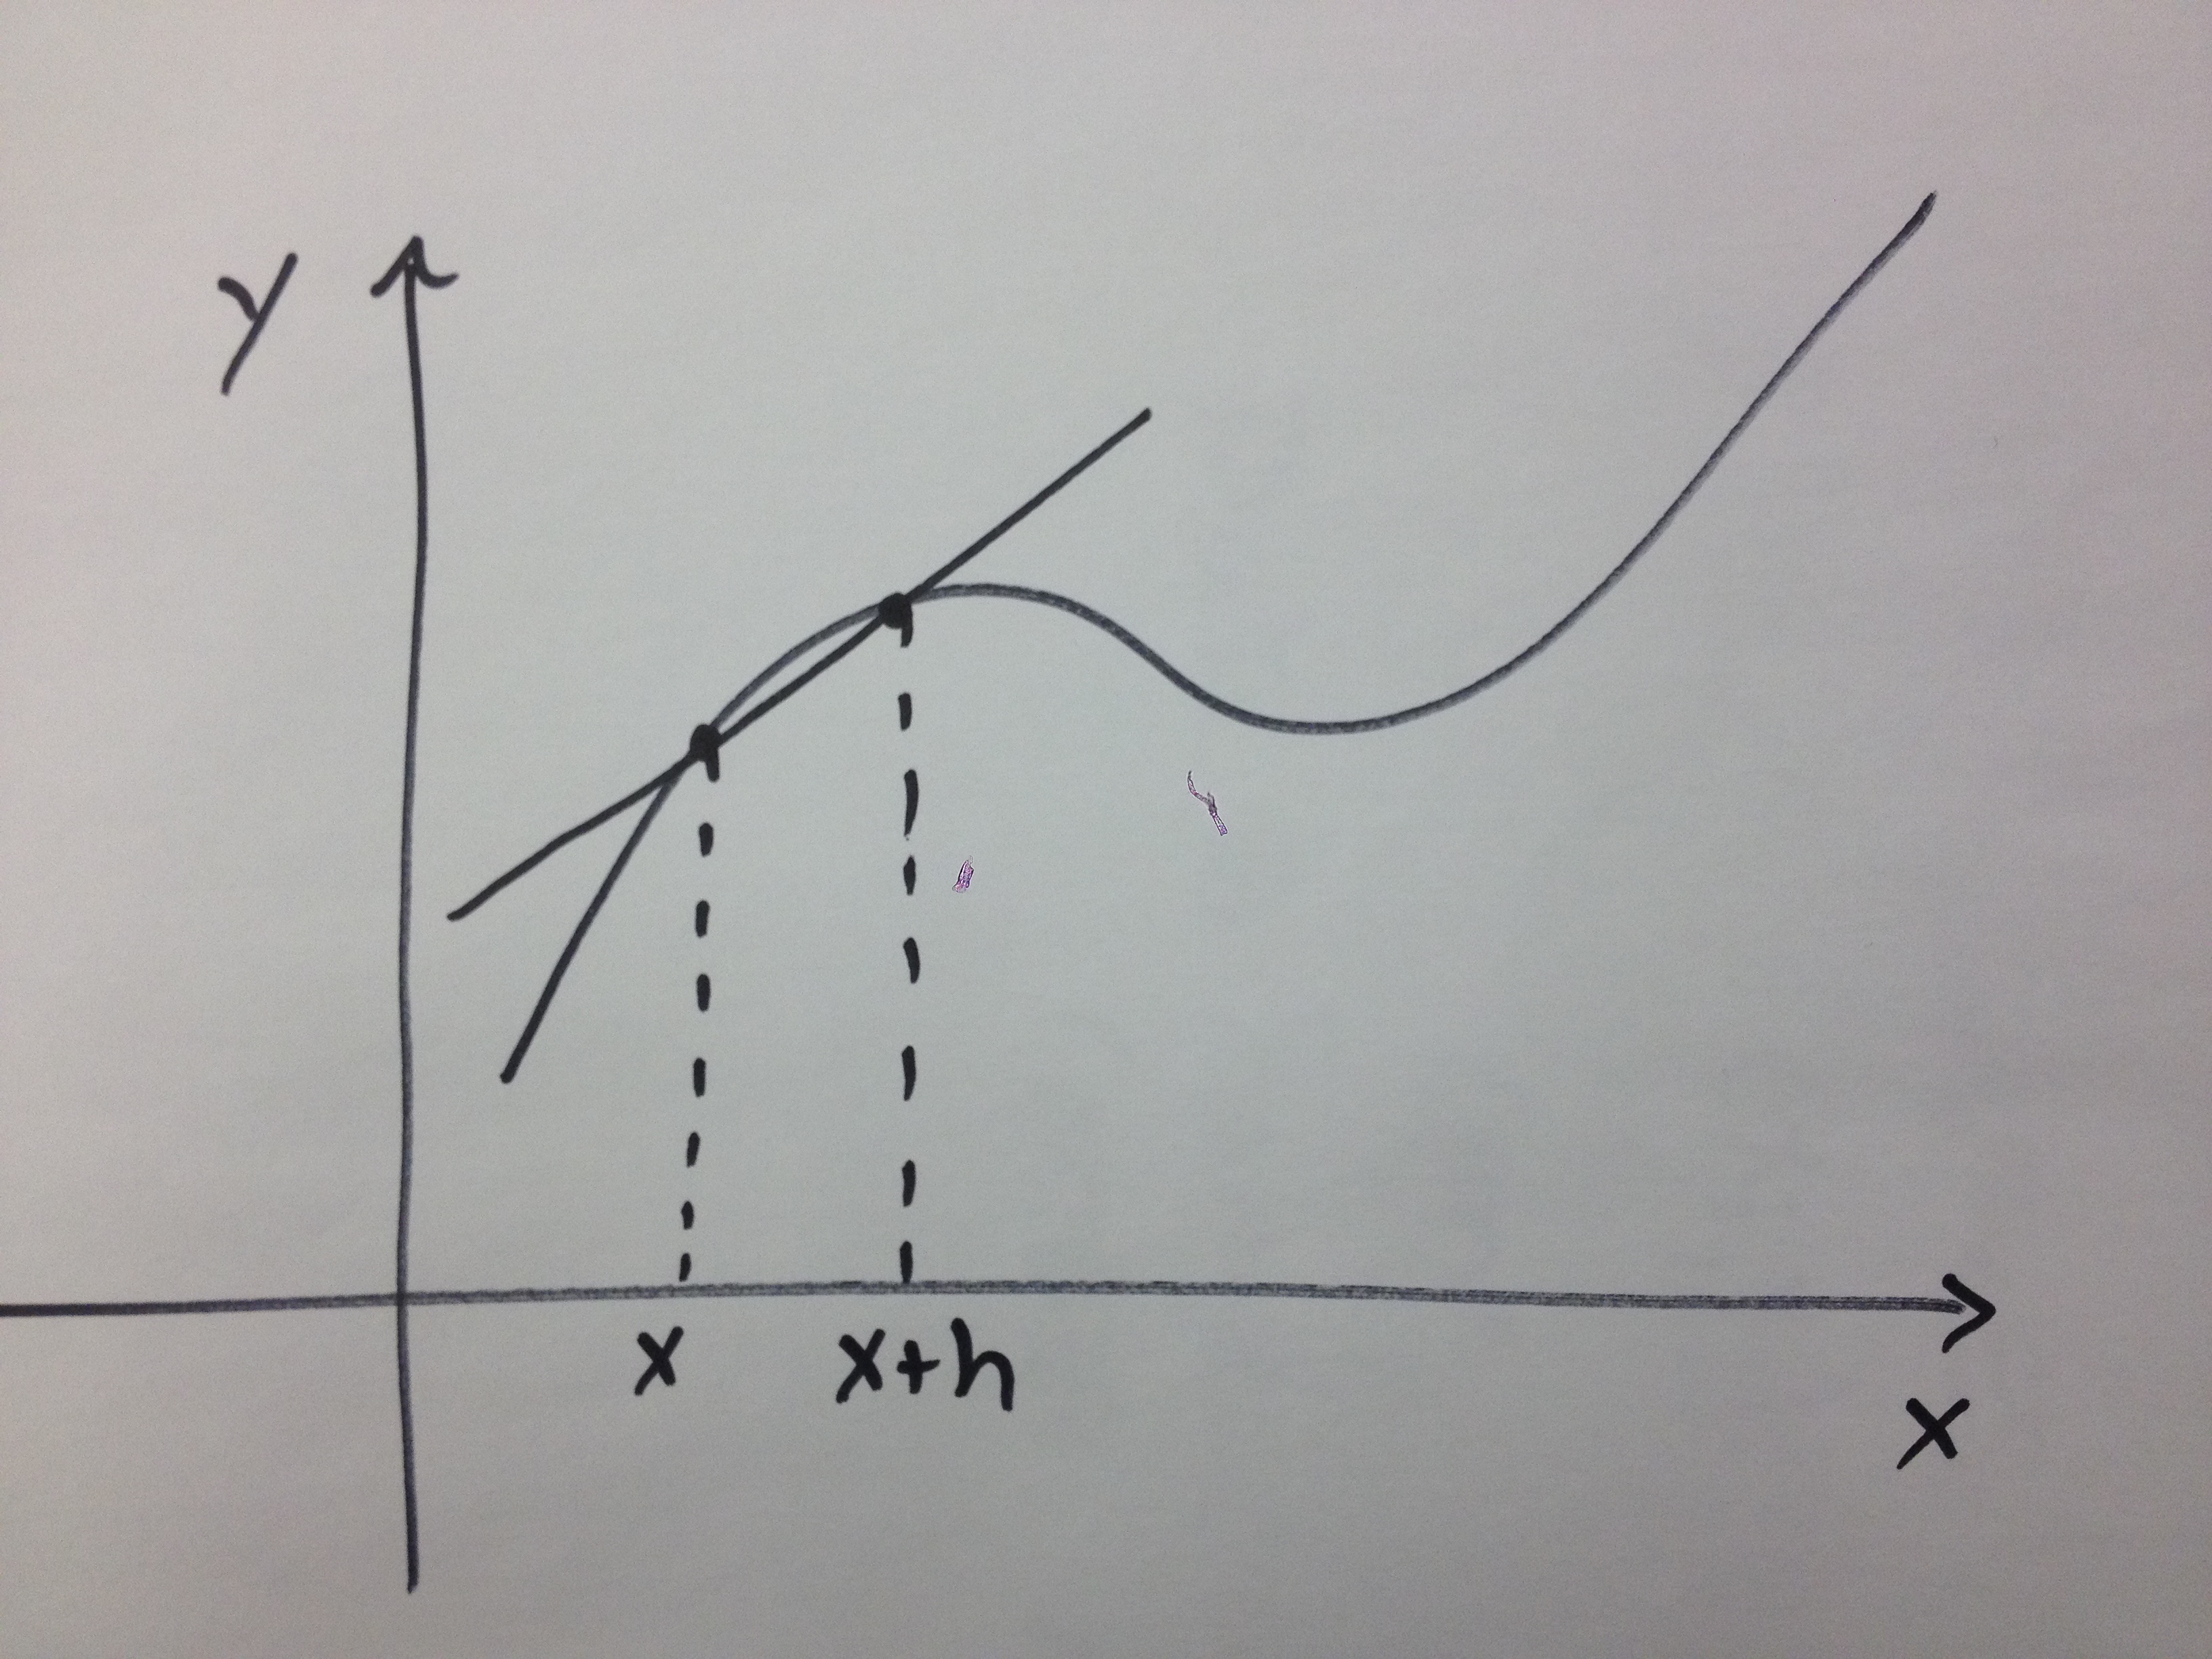
\includegraphics[width=6cm]{figs/derivative}
\caption{The derivative as a limit.}
\end{marginfigure}

What if I give you a derivative, and ask you to figure out the function that it came from? Now you are finding the anti-derivative. However, this language is not always used, and many people refer to this as the indefinite integral or just the integral. In my opinion, this is unfortunate since it presupposes the fundamental theorem of calculus, which probably means you didn't even realize that this was a cool idea!

\begin{enumerate}
\item Create a table of the five fundamental functions $x^n$, $\sin(x)$, $\cos(x)$, $\exp(x)$, and $\ln(x)$. List both their derivatives and their anti-derivatives. Include in your table at least one other example.
\item Consider the sketch of the function below. Now try to sketch the derivative and an anti-derivative.
\end{enumerate}

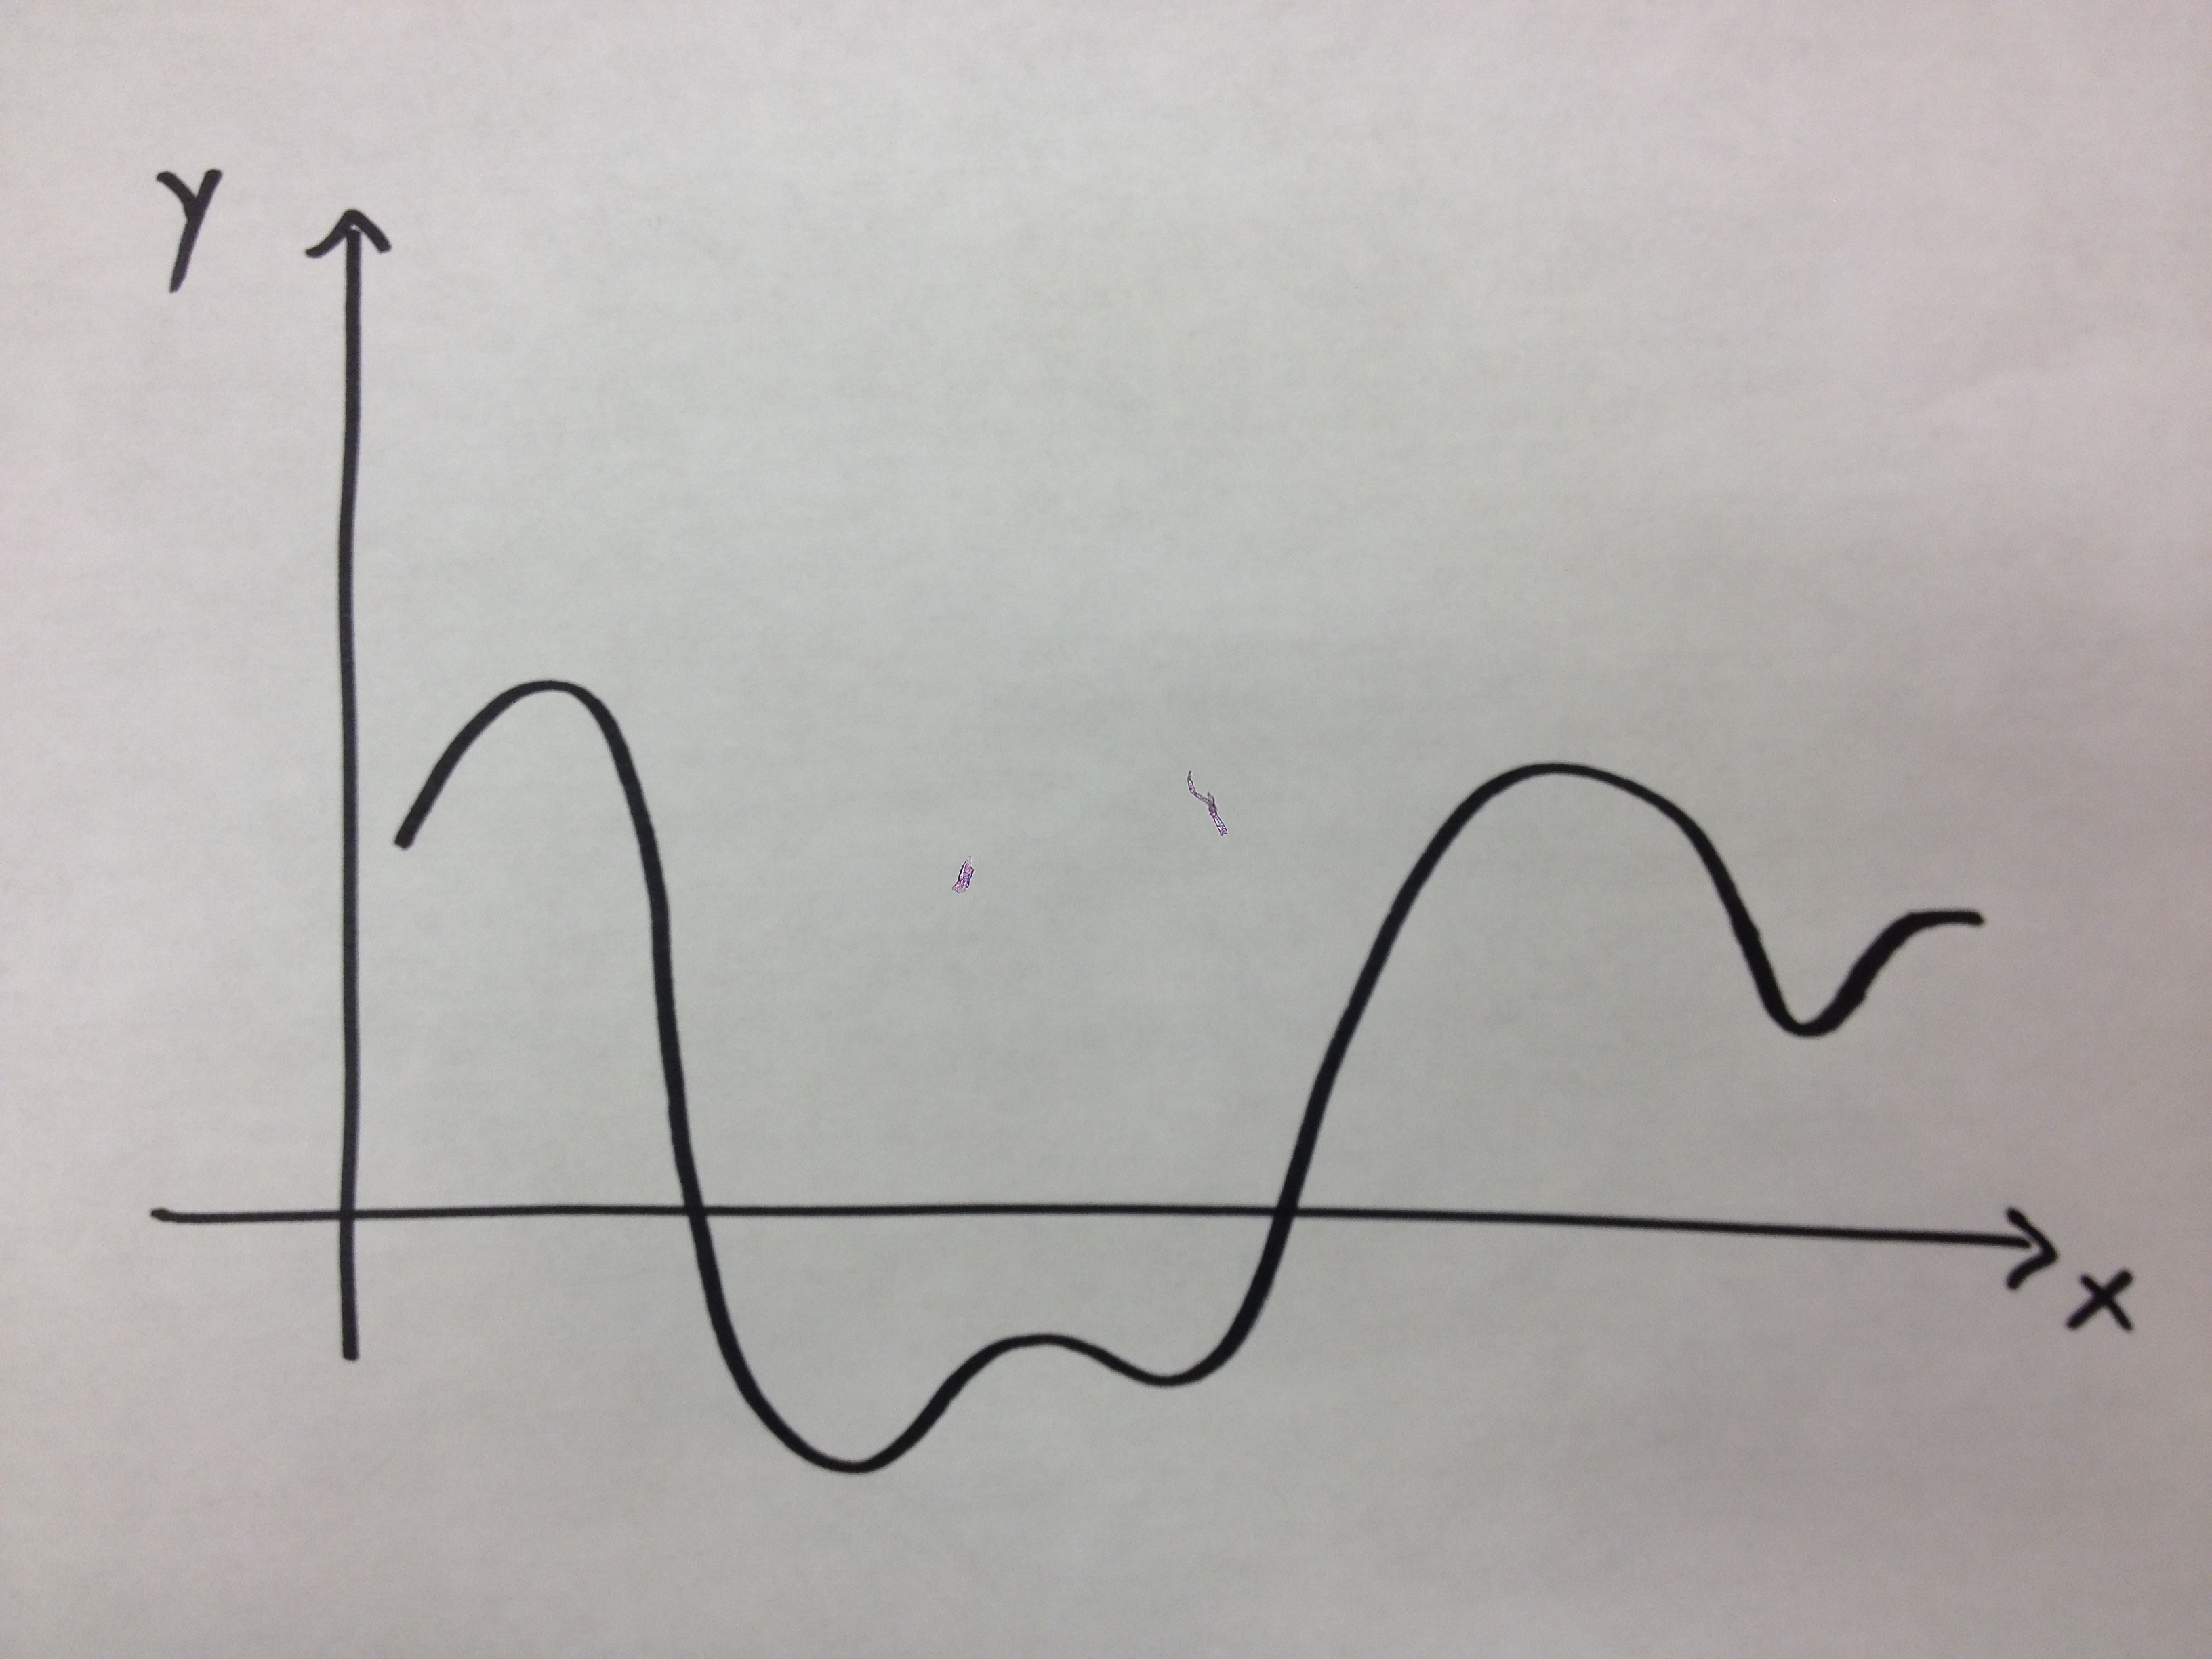
\includegraphics[width=6cm]{figs/crazyfunction}

Again consider an explicit function $y=f(x)$. The area of the region below the curve defined by $y=f(x)$, above the line $y=0$, and between the lines $x=a$ and $x=b$, is the definite integral of $f$ from $x=a$ to $x=b$,
\[\int_a^b f(x) \; dx  = \lim_{n \rightarrow \infty} \sum_{i=1}^n f(x_i) \Delta x_i. \]
We don't have to compute the area using limits: instead we appeal to the fundamental theorem of calculus.

\begin{marginfigure}
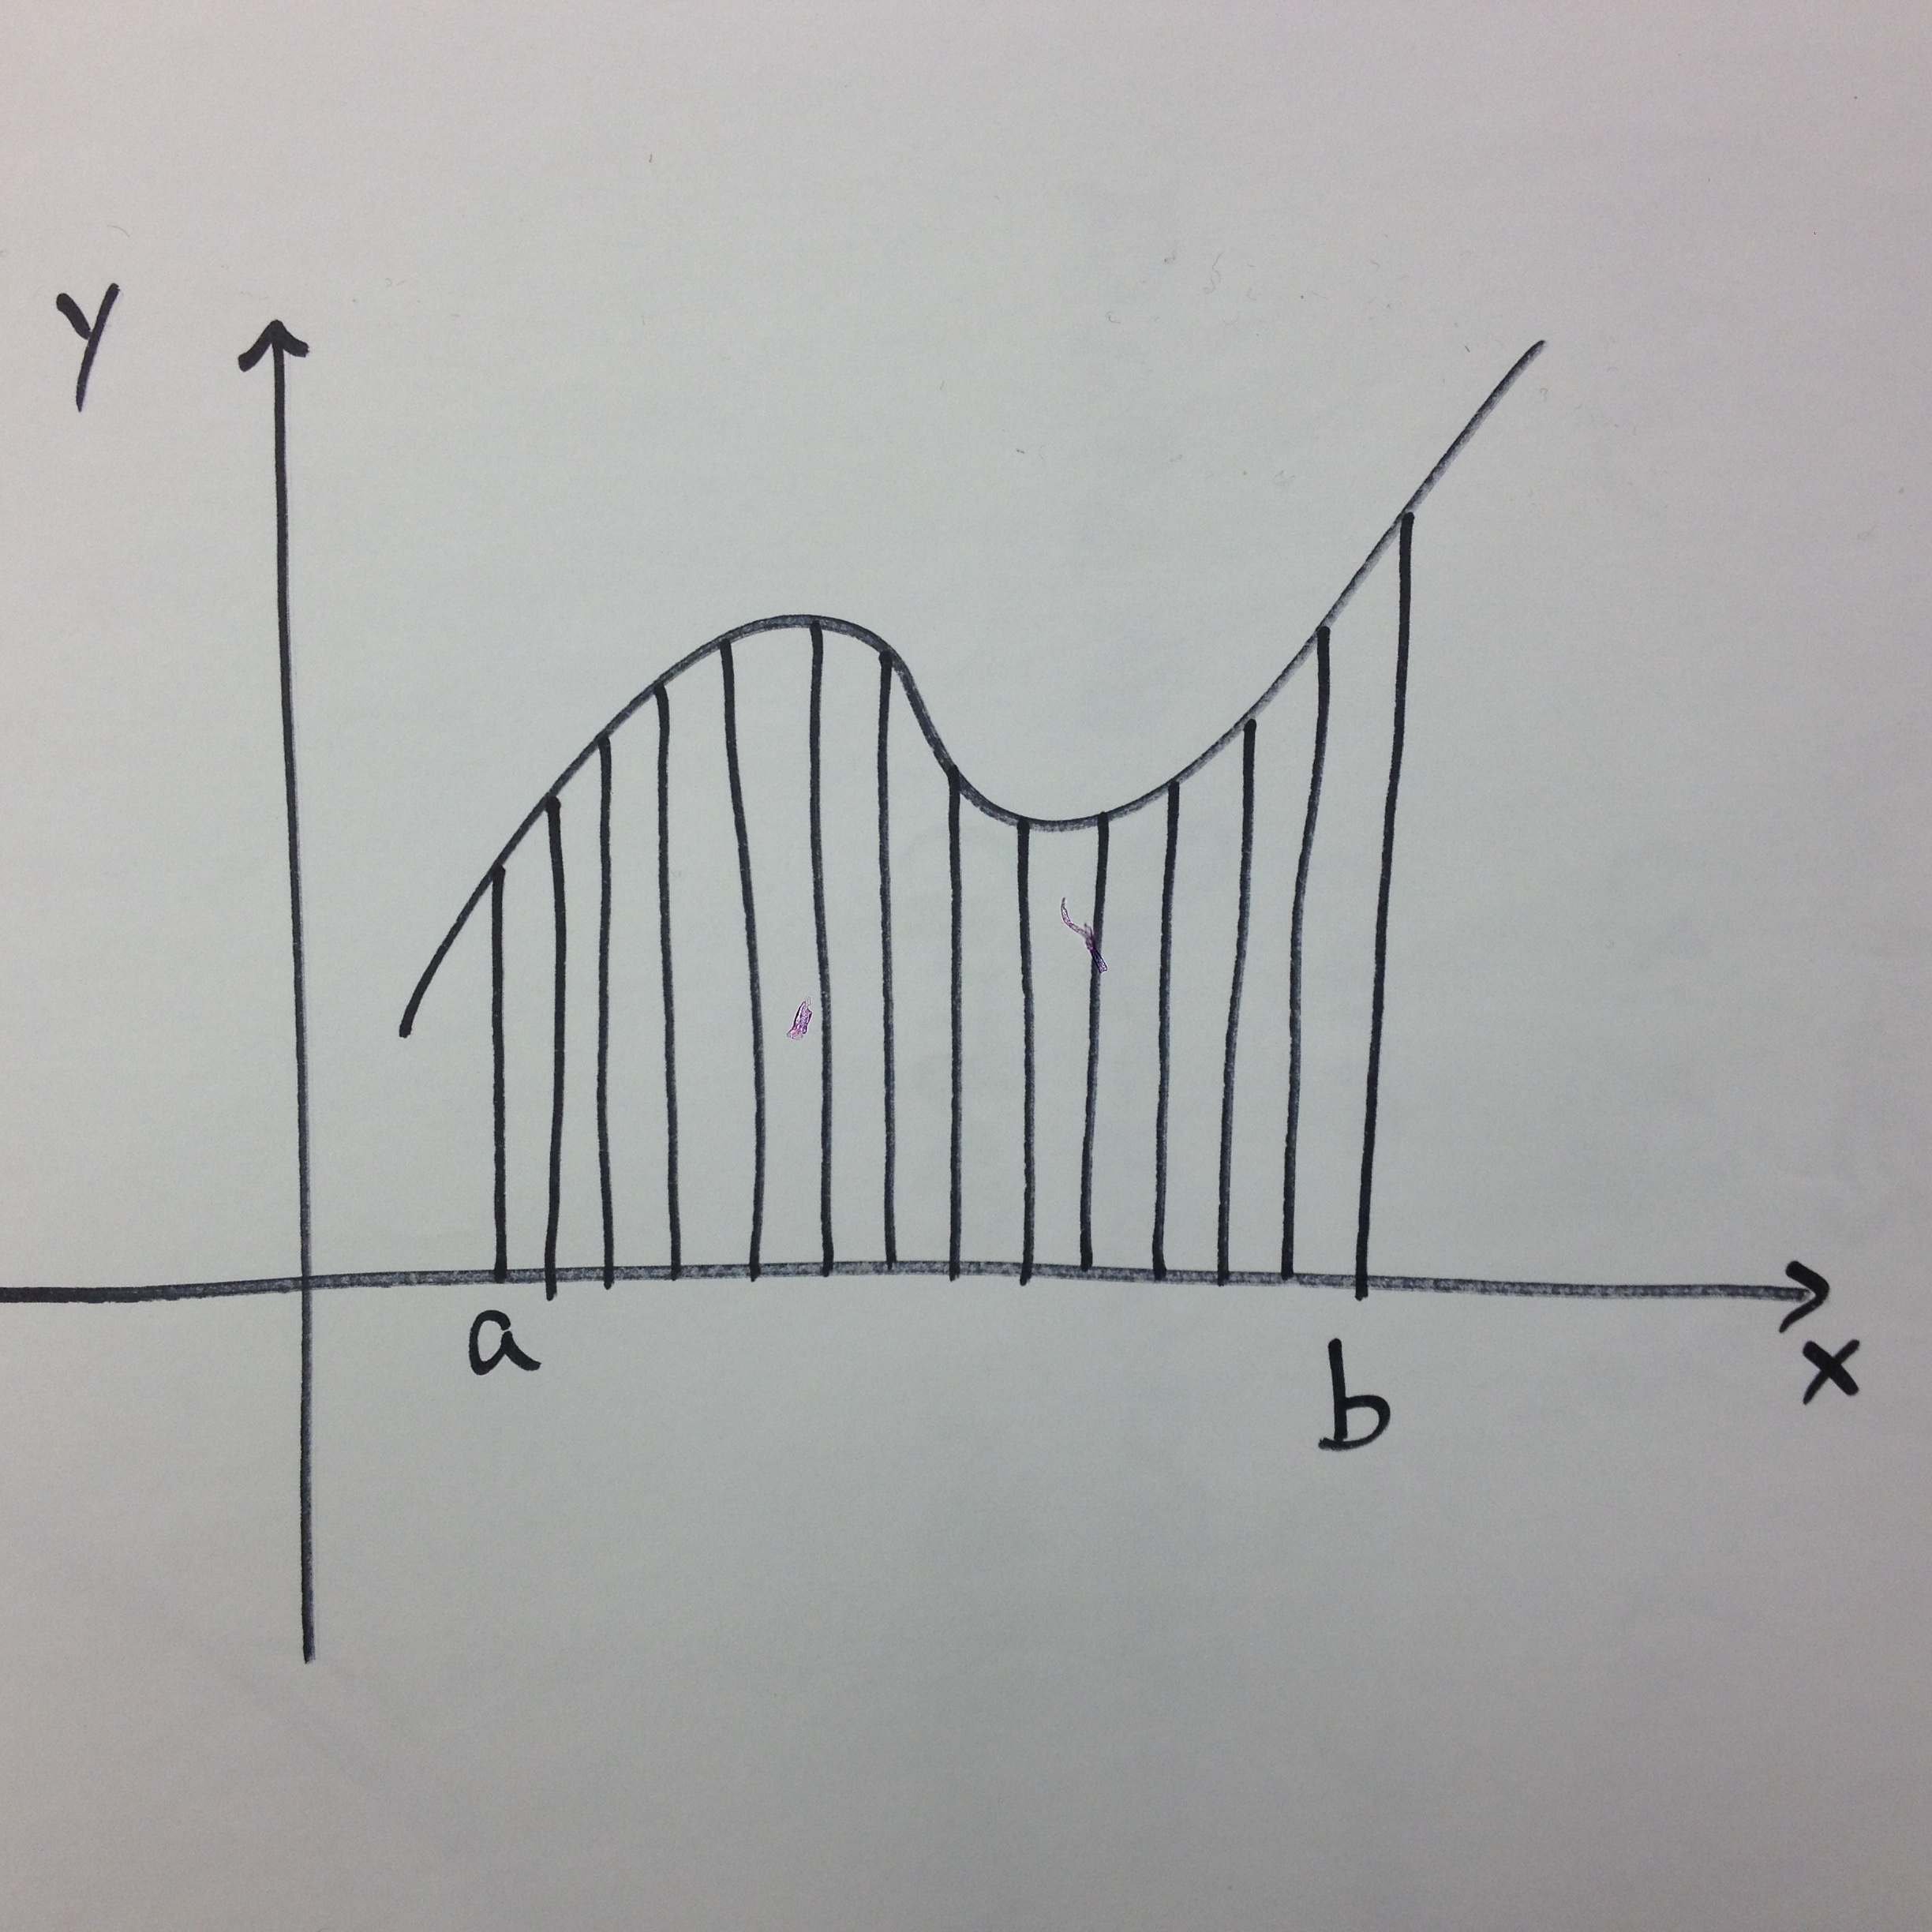
\includegraphics[width=6cm]{figs/integration}
\caption{The integral as a limit.}
\end{marginfigure}

The fundamental theorem of calculus (one of its forms anyway) states that
\[ \int_a^b f(x) \; dx = F(b) - F(a) \]
where $F$ is the anti-derivative (or indefinite integral if you insist) of $f$, or $F' = f$. In other words, integrating the slope of a function between two points gives the change in the function between the end-points. For example,
\[\int_1^2 \cos(x) \; dx = \sin(x) |_1^2 = \sin(2) - \sin(1) \]

\section{Properties and Rules of Derivatives and Integrals}
There are some key properties and rules of derivatives and integrals that we use over and over again. We include them here for completeness and ask one or two simple questions about them. These are summarized below:

\newthought{Linearity of the Derivative and Integral ($f$ and $g$ are functions, $c$ is a constant)}
\begin{eqnarray*}
(f+g)' &=& f' + g' \\
(cf)' &=& cf' \\
\int_a^b f + g \; dx &=& \int_a^b f \; dx + \int_a^b g \; dx \\
\int_a^b cf \; dx &=& c \int_a^b f \; dx
\end{eqnarray*}

\begin{enumerate}[resume]
\item Make a visual argument about why these properties are true.
\end{enumerate}

\newthought{Chain Rule and Substitution Rule}
\begin{eqnarray*}
\frac{d}{dx} f(u(x)) &=& f' (u(x)) \; u'(x) \\
\int_a^b f(u(x)) u'(x) \; dx &=& \int_{u(a)}^{u(b)} f(u) \; du
\end{eqnarray*}

\begin{enumerate}[resume]
\item Use your table of fundamental functions and the chain rule to determine the derivative of $(x^3-1)^{100}$.
\item Use your table of fundamental functions and the substitution rule to evaluate $\int_0^4 \sqrt{2x+1} \; dx$.
\end{enumerate}
 
\newthought{Product Rule and Integration by Parts}
\begin{eqnarray*}
\frac{d}{dx} f(x) g(x) &=& f \frac{dg}{dx} + g \frac{df}{dx} \\
\int_a^b f(x) g'(x) \; dx &=& f(x) g(x) |_a^b - \int_a^b g(x) f'(x) dx
\end{eqnarray*}

\begin{enumerate}[resume]
\item Use your table of fundamental functions and the product rule to determine the derivative of $\sqrt{x} (1-x)$.
\item Use your table of fundamental functions and integration by parts to determine $\int_1^2 x \exp(-x) \; dx$.
\end{enumerate}

\section{Areas enclosed by curves}

Single-variable calculus gives us the tools to compute the area of regions bounded by curves. Consider the region bounded on top by $y=f(x)$, on the bottom by $y = g(x)$, and on the sides by $x=a$ and $x=b$. Appealing to the properties of integrals, the area of this region is
\[\int_a^b f(x) - g(x) \; dx \]
We should note that integration will return a signed area. For example, the integral will be negative if the value of the function $g$ is greater than that of $f$.

\begin{marginfigure}
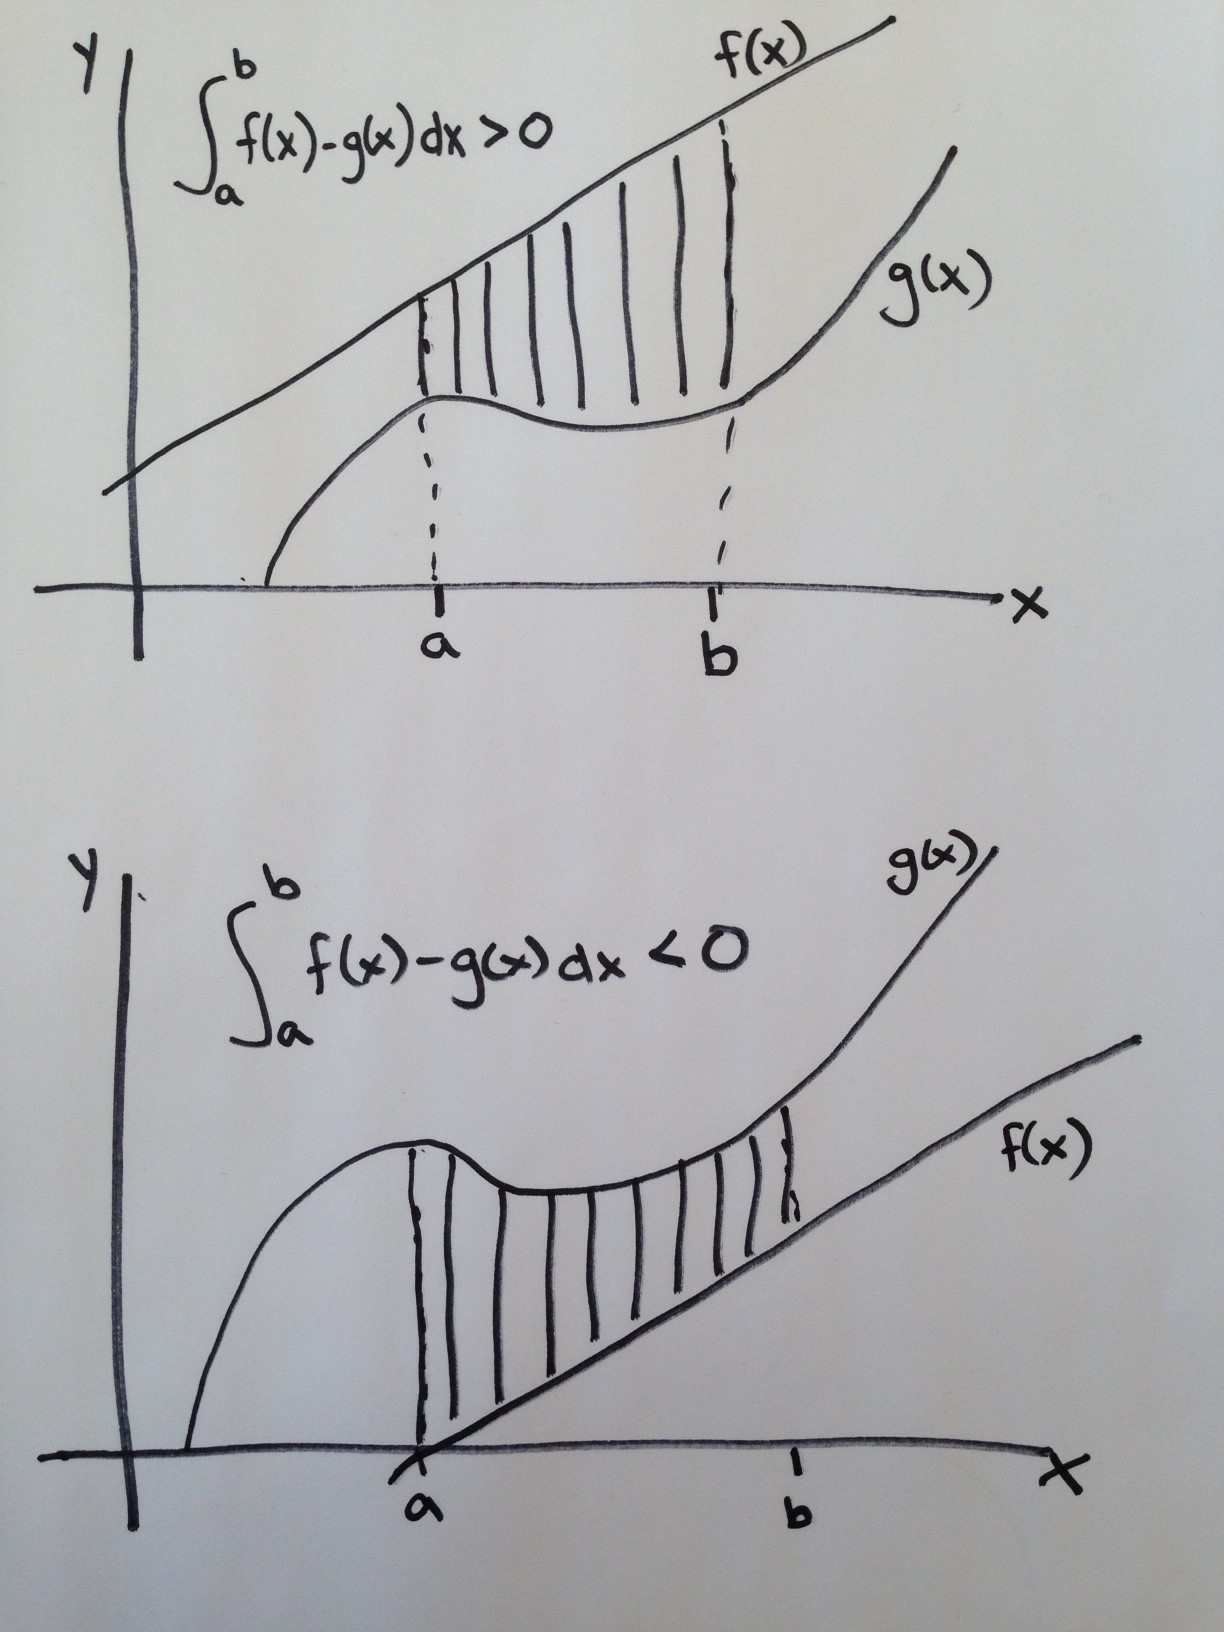
\includegraphics[width=6cm]{figs/signedarea}
\caption{The area defined by integration can be positive or negative.}
\end{marginfigure}

\begin{enumerate}[resume]
\item Recall some of the explicit functions you used to describe curves generated by taking sections through fruit, vegetables, or manufactured objects. Propose an integral that would determine the cross-sectional area of the section, and evaluate it.
\item Consider the family of functions defined by the power law, $y = x^n, n = 1,2,3,\ldots$. Propose an integral that would determine the area enclosed on the top by $y=d$, on the bottom by $y = x^n$, on the left by $x=0$, and on the right by the intersection of the top and bottom functions. Evaluate it and graph the enclosed area as a function of the parameter $d$. Use a log-log plot and interpret the result.
\end{enumerate}

\begin{marginfigure}
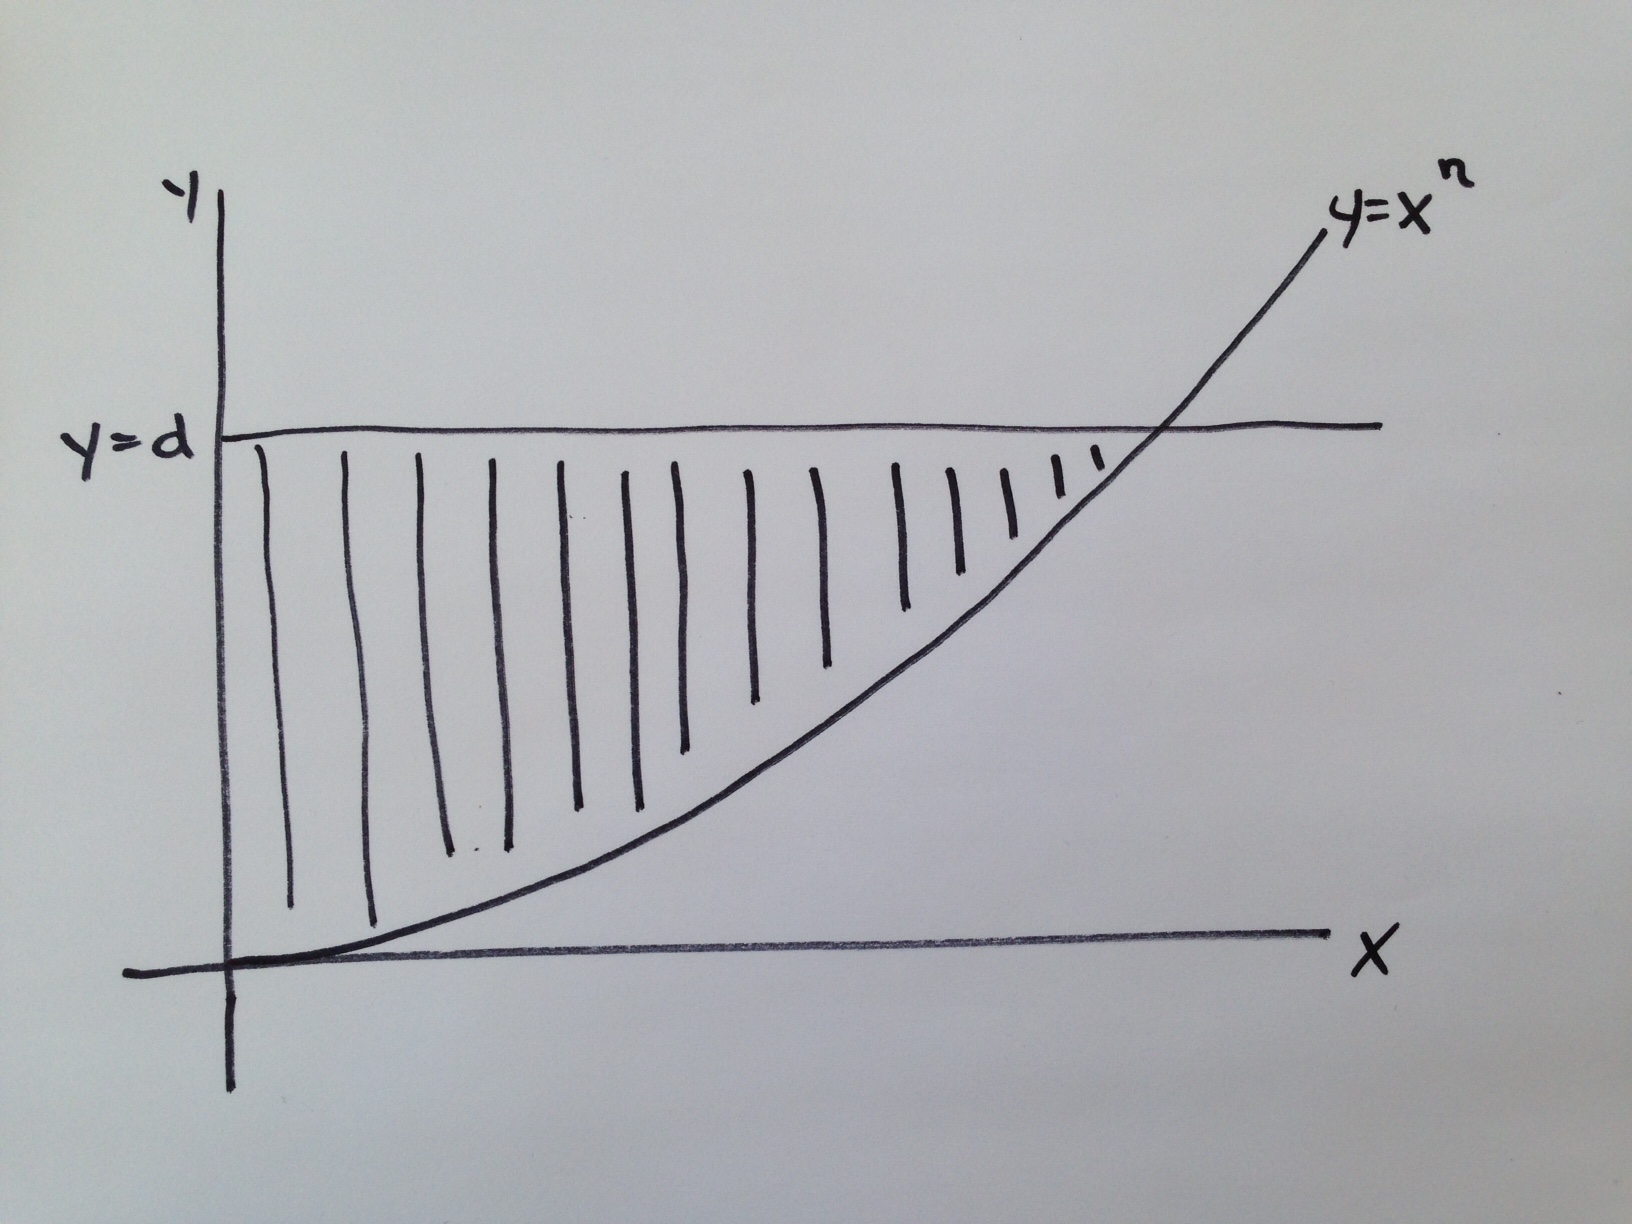
\includegraphics[width=6cm]{figs/areadepth}
\caption{Imagine this is the cross-section of a boat with different waterlines.}
\end{marginfigure}

\section{Functions of several variables}
In Shapes I we met functions of several variables, e.g. $f(x,y)$. In this section we will think about the notion of derivative or integral of such functions. We will rely on visual representations of the surface defined by $z=f(x,y)$. 

\subsection{Derivatives}
Consider a function of two variables $f(x,y)$. At any point on the surface, $(a,b,c)$, we can ask about the slope of the tangent line in the x-direction and in the y-direction. In the first case, we intersect the surface with the plane $y=b$ and consider the rate of change of $f$ in the x-direction only. In the second case, we use the plane $x=a$ and consider the rate of change of $f$ in the y-direction only. There are therefore two fundamental derivatives, 

$\frac{\partial f}{\partial x}$: {\it partial derivative of f with respect to x}

$\frac{\partial f}{\partial y}$: {\it partial derivative of f with respect to y}

\begin{marginfigure}
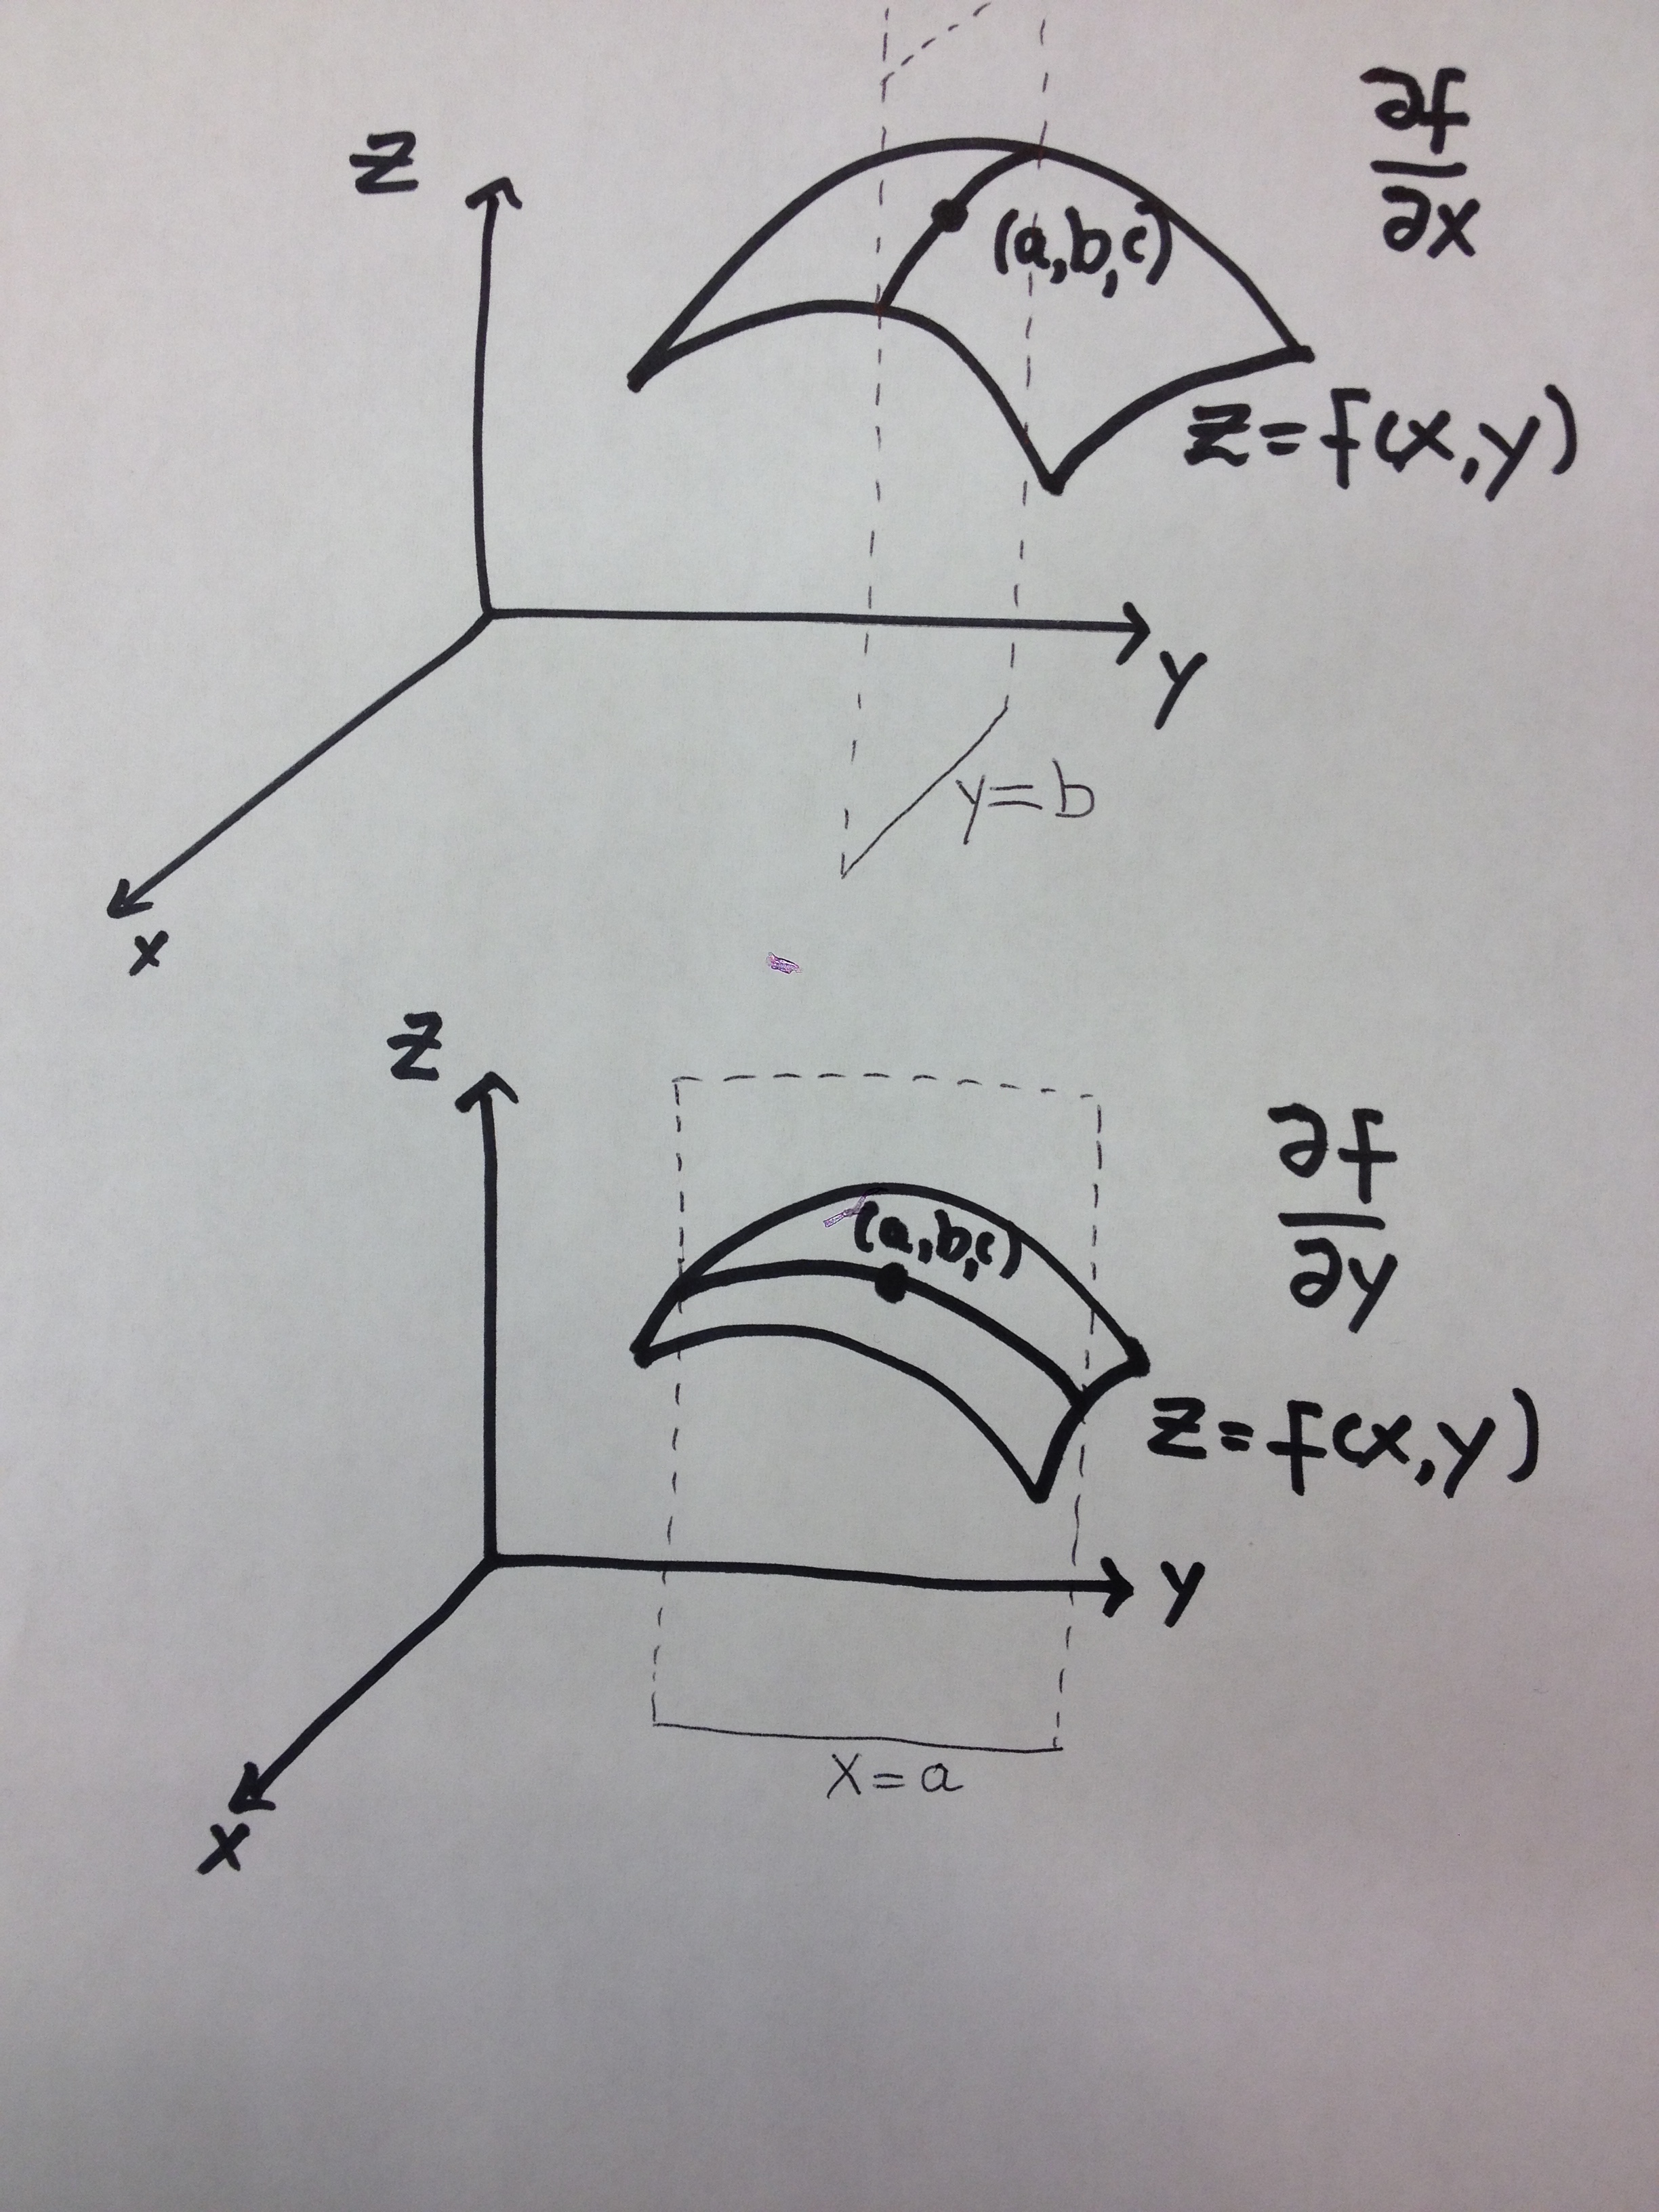
\includegraphics[width=6cm]{figs/partial_derivs}
\caption{Partial derivatives of a function of two variables.}
\end{marginfigure}

In each case we compute the derivative with respect to one variable by holding the other one fixed, i.e. treating it as a constant.

\begin{enumerate}[resume]
\item Evaluate $\frac{\partial f}{\partial x}$ and $\frac{\partial f}{\partial y}$ for $f(x,y) = x^2 \sin(xy^2)$.
\end{enumerate}

We can also evaluate higher-order derivatives, but now there are several possibilities. We could take two derivatives with respect to x. We could take two derivatives with respect to y. Or we could take a derivative with respect to x and then with respect to y, and vice versa. The notation for each of these is:

\[\frac{\partial}{\partial x} \frac{\partial f}{\partial x} = \frac{\partial^2 f}{\partial x^2} \]
\[\frac{\partial}{\partial y} \frac{\partial f}{\partial y} = \frac{\partial^2 f}{\partial y^2} \]
\[\frac{\partial}{\partial y} \frac{\partial f}{\partial x} = \frac{\partial^2 f}{\partial y \partial x} \]
\[\frac{\partial}{\partial x} \frac{\partial f}{\partial y} = \frac{\partial^2 f}{\partial x \partial y} \]

\begin{enumerate}[resume]
\item Evaluate all four second-order derivatives of $f(x,y) = x^2 \sin(xy^2)$.
\end{enumerate}

Under very gentle conditions it is generally true that the mixed partial-derivatives are always equal, i.e. 
\[ \frac{\partial^2 f}{\partial y \partial x} = \frac{\partial^2 f}{\partial x \partial y} \]

\begin{enumerate}[resume]
\item Review the article on partial derivative at {\it http://mathworld.wolfram.com/PartialDerivative.html} Under what conditions on the function $f$ are the mixed partial derivatives equal?
\end{enumerate}

There is no reason not to extend the idea of partial derivatives to functions of many variables.

\begin{enumerate}[resume]
\item How many second-order derivatives are there of $f(x,y,z)$?
\end{enumerate}

\section{Areas as double integrals}

This is going to seem really weird and stupid the first time you read it. Come back to it in a week and see how it feels then.

Consider a rectangle enclosed by $x=a$, $x=b$, $y=c$, and $y=d$. The area of the rectangle according to calculus is
\[\int_a^b d - c \; dx \]
which (fortunately) evaluates to $(b-a)(d-c)$. Consider the integrand, $d-c$. According to the fundamental theorem of calculus, this difference could be expressed as an integral
\[d - c = \int_c^d dy \]
which is at the very least an interesting thing to do. Replacing this expression into the earlier one means the area of the rectangle could be expressed as a {\it double integral}
\[\int_a^b \int_c^d dy dx \]
A word on notation: the inner integral is with respect to y, with limits defined by $y=c$ and $y=d$. The outer integral is with respect to $x$, with limits defined by $x=a$ and $x=b$. Since we could have expressed the area as
\[\int_c^d b - a \; dy \]
the area of the rectangle can also be expressed as the {\it double integral}
\[\int_c^d \int_a^b dx dy \]
Notice how the order of integration and corresponding limits have changed, but (presumably) the result hasn't.

Now consider a region enclosed by two functions $y = f(x)$ and $y=g(x)$ and two lines $x=a$ and $x=b$. Using the same reasoning, the area of this enclosed region can be expressed as a double integral
\[\int_a^b \int_{f(x)}^{g(x)} dy dx \]

\begin{enumerate}[resume]
\item Sketch the regions of integration and compute the area of the enclosed region by evaluating the double integral.
\begin{enumerate}
\item $ \int_0^1 \int_0^x dy dx $
\item $ \int_0^{\pi/2} \int_0^{\sin x} dy dx $
\item $ \int_1^2 \int_0^{\ln x} dy dx $
\end{enumerate}
\end{enumerate}

\begin{marginfigure}
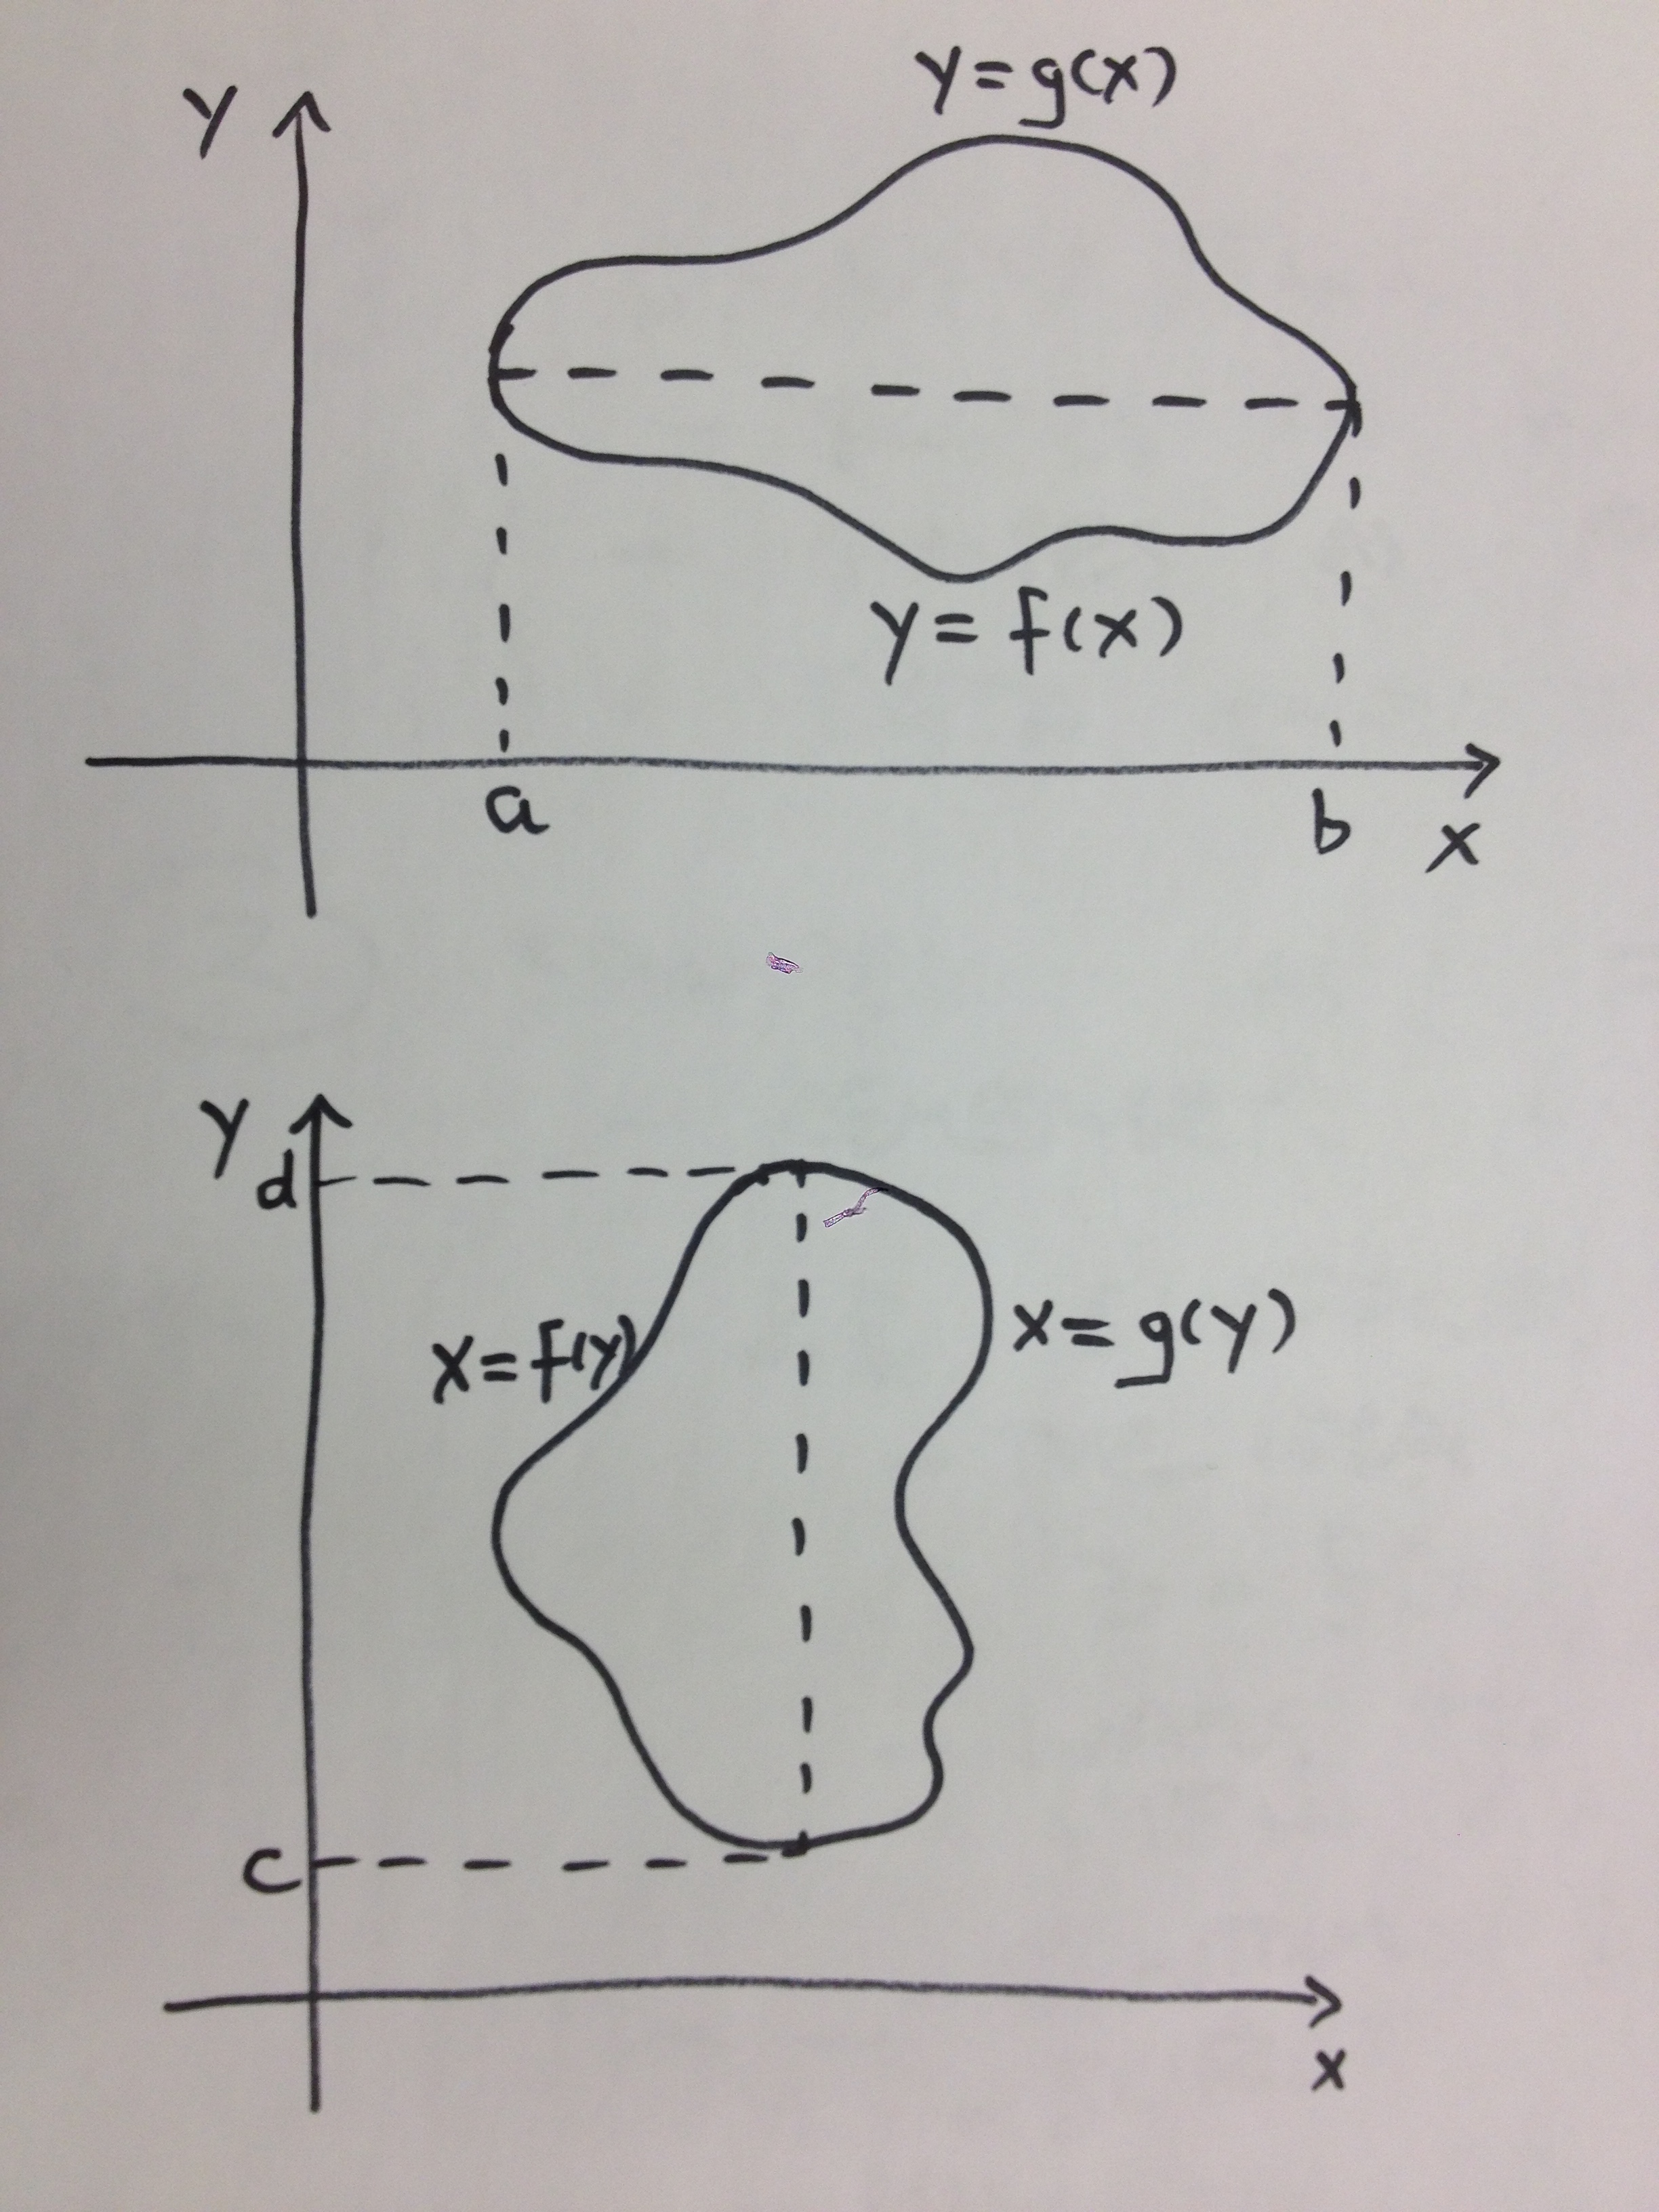
\includegraphics[width=6cm]{figs/simpleregions}
\caption{Simple regions in the plane that enclose areas.} 
\end{marginfigure}

What if the region must be described by two functions $x=f(y)$ and $x = g(y)$, and two lines $y=c$ and $y=d$. In this case we would integrate with respect to $x$ first, and then with respect to $y$,
\[ \int_c^d \int_{f(y)}^{g(y)} dx dy \]

\begin{enumerate}[resume]
\item Sketch the regions of integration and compute the area of the enclosed region by evaluating the double integral.
\begin{enumerate}
\item $ \int_0^1 \int_y^{2-y} dx dy $
\item $ \int_0^4 \int_{y/2}^2 dx dy $
\item $ \int_0^1 \int_y^{\exp y} dx dy $
\end{enumerate}
\item Consider the following region. Express the region as a union of simple regions, and compute the area using double integrals.
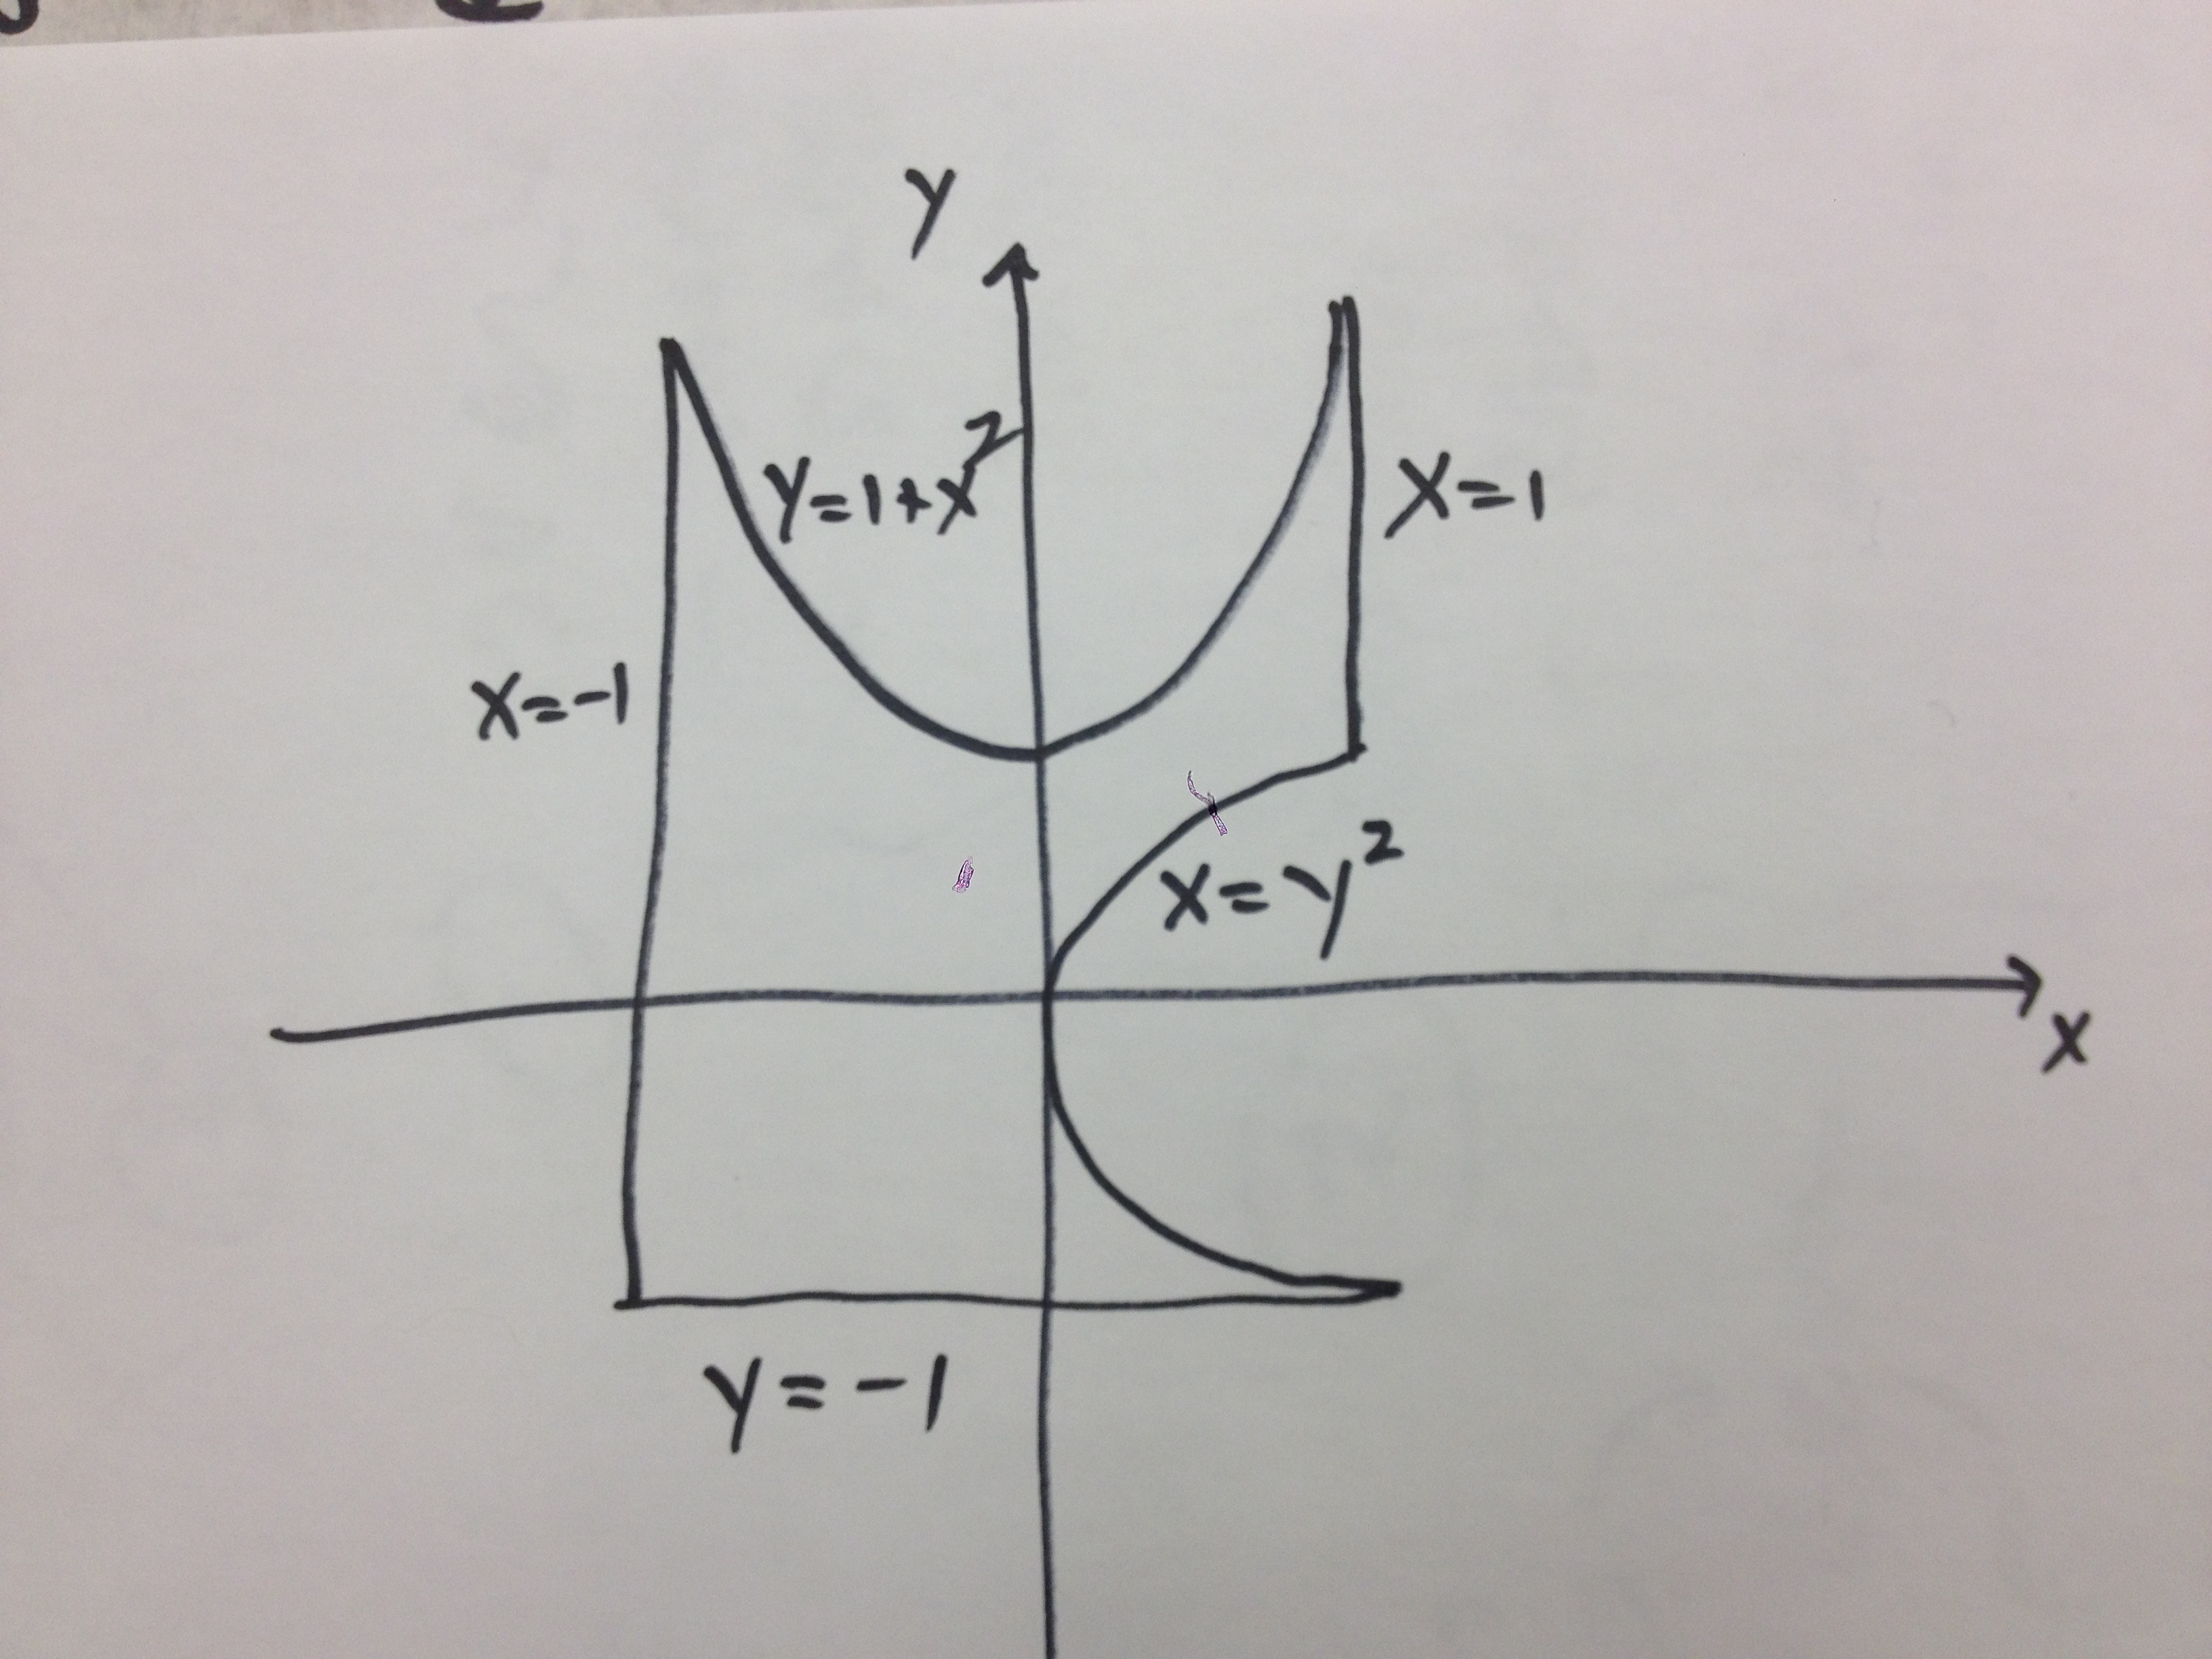
\includegraphics[width=6cm]{figs/weirdregion}
\end{enumerate}

\section{Volumes enclosed by surfaces defined by $z=f(x,y)$}

Consider the volume enclosed by the surfaces defined by $z=f(x,y)$, $z = 0$, $x=a$, $x=b$, $y=c$, and $y=d$.
How would we compute the volume of this region? One option would be to slice the surface up in sections parallel to one of the coordinate planes. For example, if we make a slice at $x=x_1$, then each planar region is bounded by $z = f(x_1,y)$, $y=c$, and $y=d$. The area of the enclosed region is therefore
\[ \int_c^d f(x_1,y) \; dy \]

\begin{marginfigure}
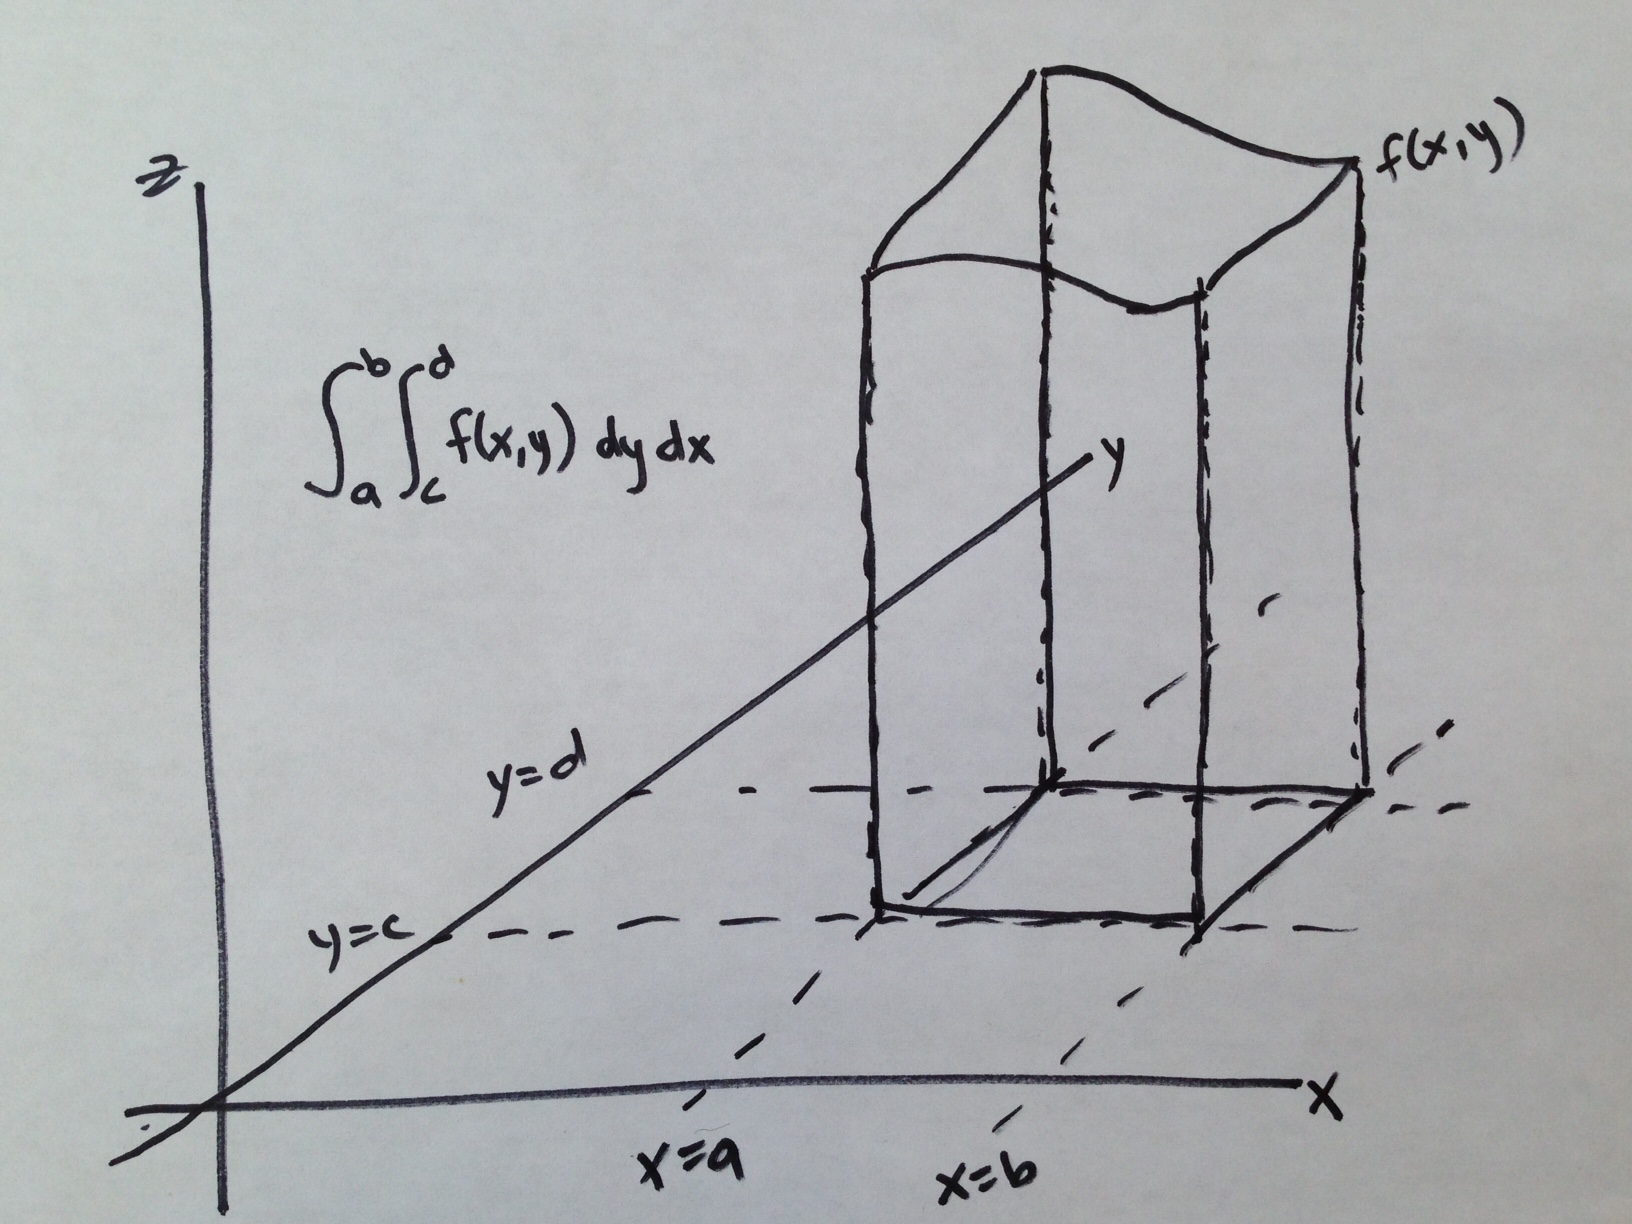
\includegraphics[width=6cm]{figs/volumerectangular}
\caption{Volume defined as a double integral over a rectangle in the plane.}
\end{marginfigure}

If we repeat this for different values of $x$, then we could compute the area of each cross-section as a function of $x$
\[ area(x) = \int_c^d f(x,y) \; dy \]
What happens if we now integrate the area function from $x=a$ to $x=b$? We should get a volume, and it should be the volume of the original enclosed region,
\[ Volume = \int_a^b area(x) \; dx = \int_a^b \int_c^d f(x,y) \; dy dx \]
As we saw earlier, it shouldn't matter whether we change the order of integration.

Notice that the region of integration is the rectangle in the plane defined by $(x,y) \in [a,b] \times [c,d]$. There is no reason that the integral can't be computed over more general regions. In general we will use the coordinate-free notation
\[ \iint\limits_D f \; dA \]
to define the double integral of a function over a general region $D$ in the plane.

\begin{marginfigure}
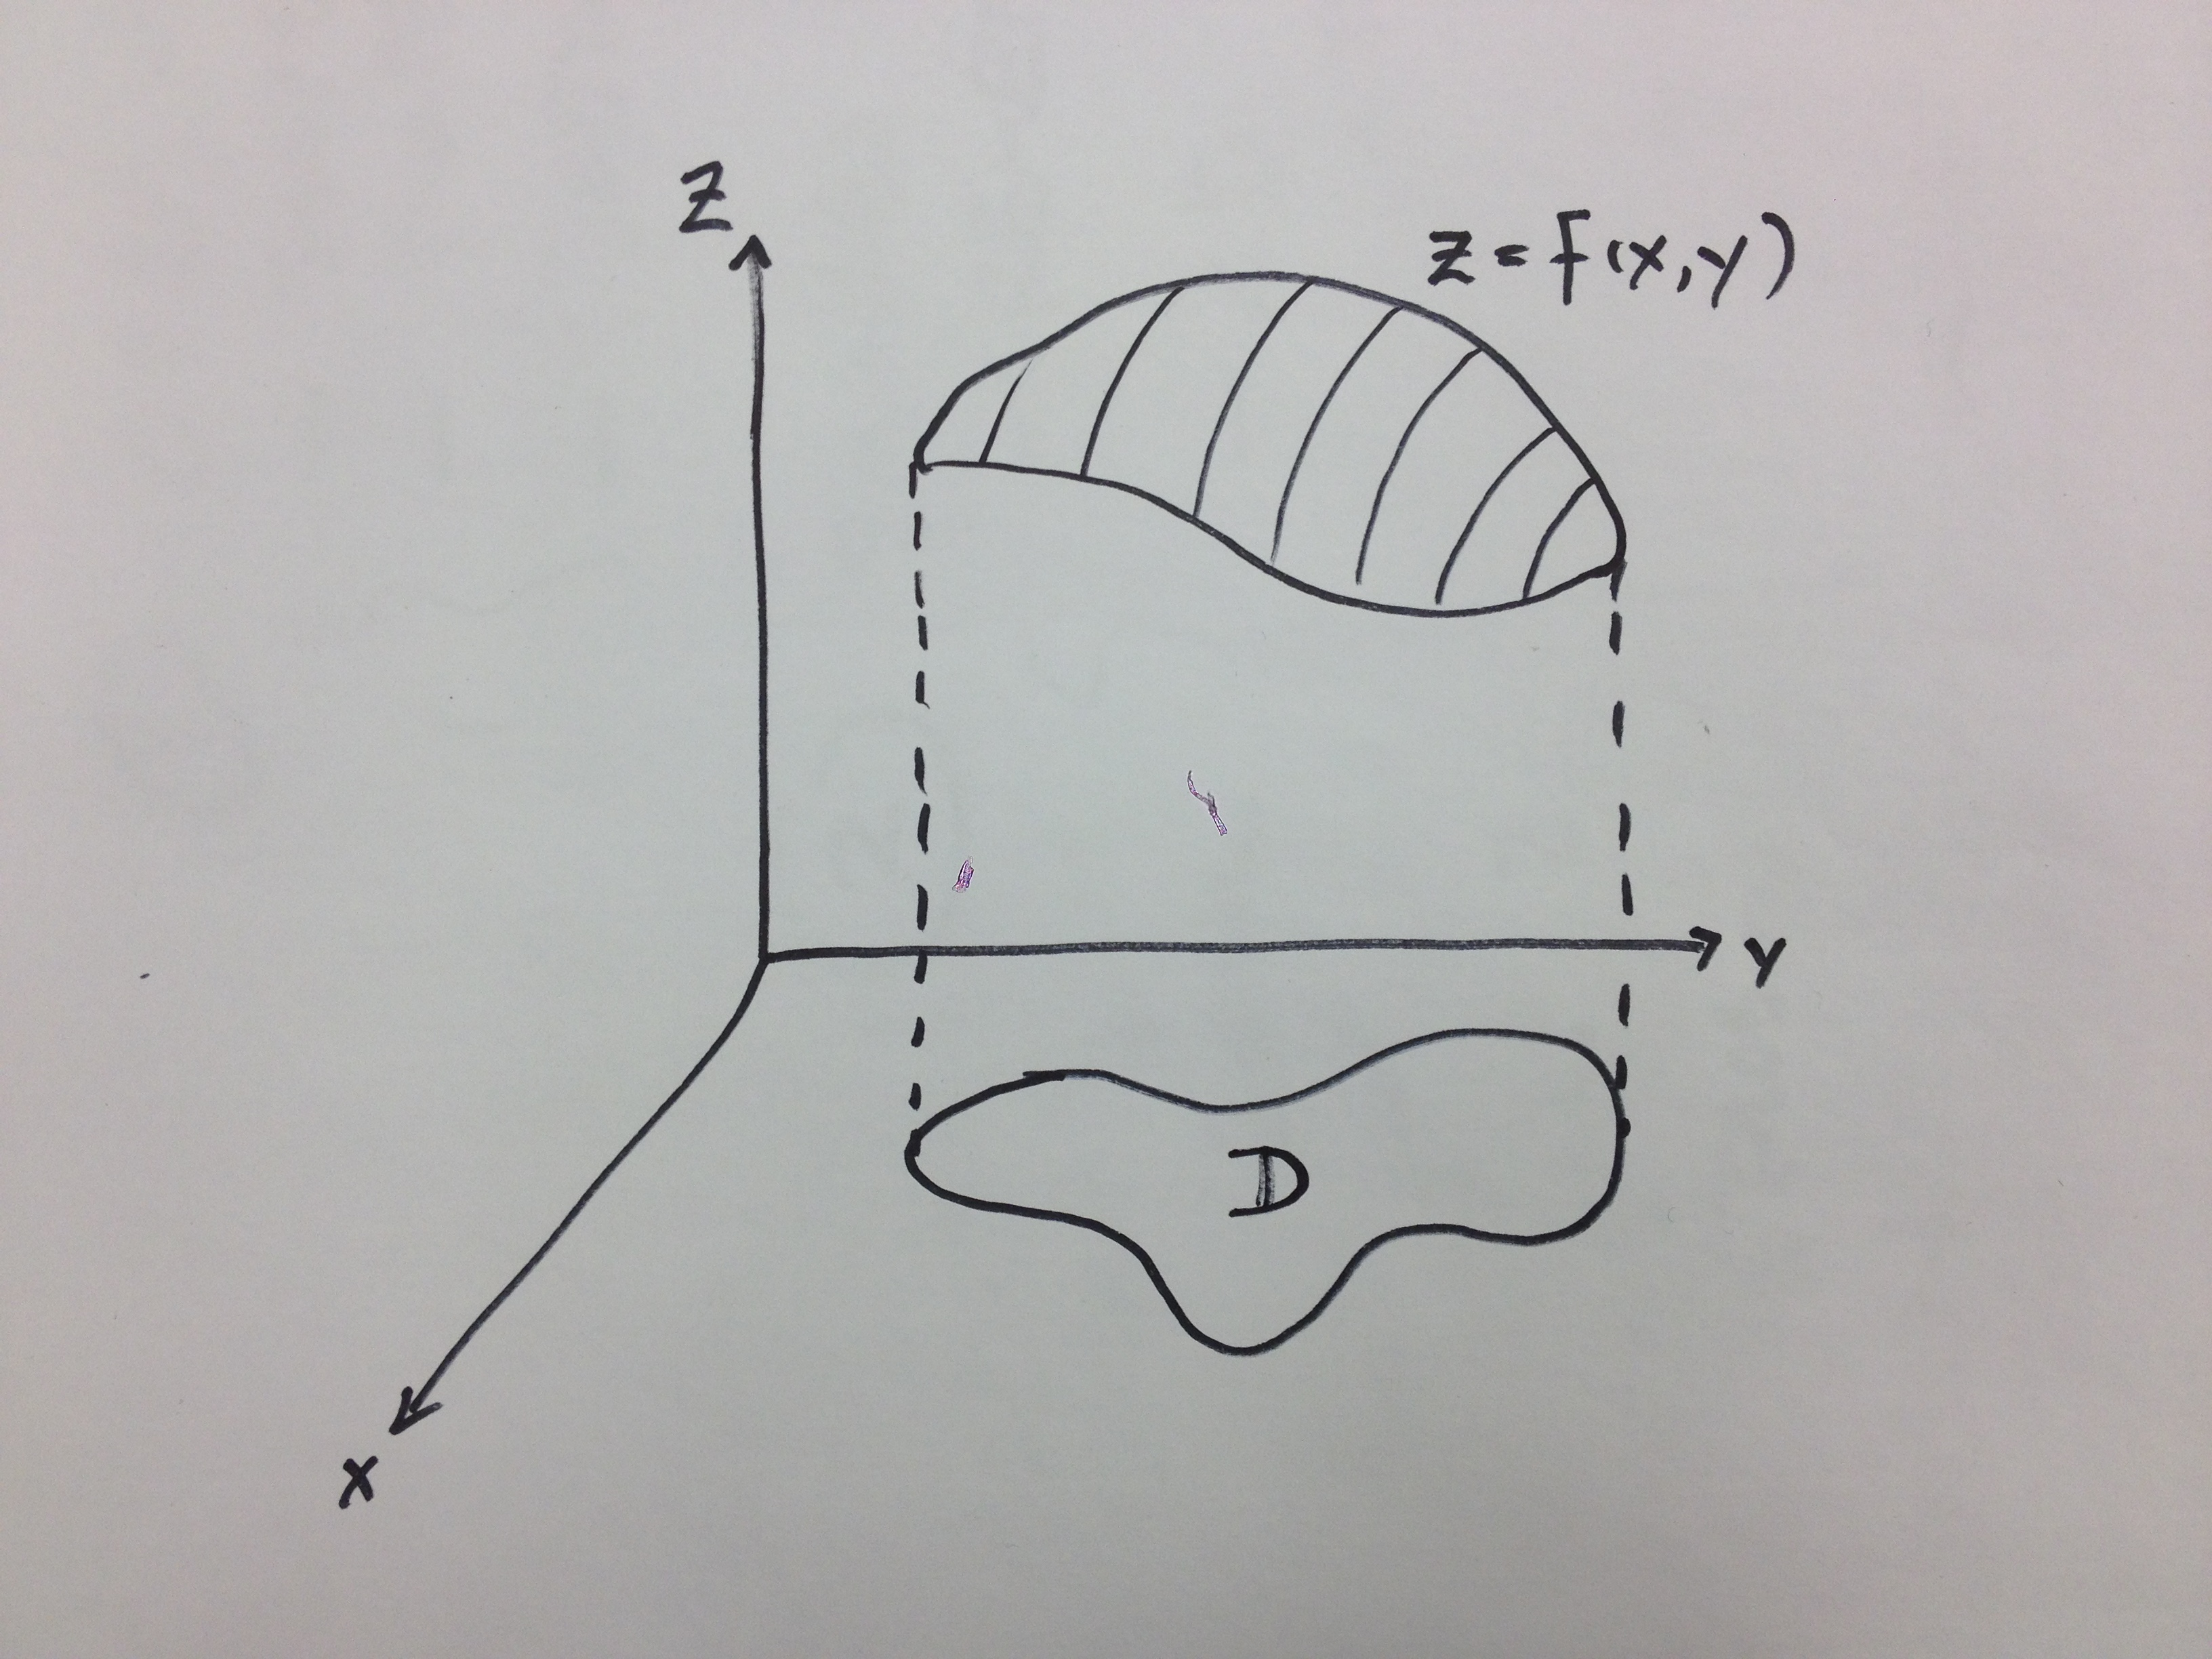
\includegraphics[width=6cm]{figs/volumegeneral}
\caption{Volume defined as a double integral over a general region in the plane.}
\end{marginfigure}

\begin{enumerate}[resume]
\item Sketch the following regions of integration in the plane, and evaluate the double integral.
\begin{enumerate}
\item $\iint\limits_D  \frac{4y}{x^3+2} \; dA, \; D = \{(x,y) | 1 \le x \le 2, 0 \le y \le 2x\} $
\item $\iint\limits_D x \cos y \; dA, $ \; D is bounded by $y=0, y = x^2, x = 1$ 
\end{enumerate}
\item Visualize the following solids and compute their volume using a double integral.
\begin{enumerate}
\item Bounded by the planes $x = 0$, $y=0$, $z=0$, and $x+y+z=1$.
\item Under the paraboloid $z = x^2 + y^2$ and above the region bounded by $y=x^2$ and $x=y^2$.
\end{enumerate}
\end{enumerate}

In the same way that we could view area as a single or double integral (with the appropriate integrand), we can think of volume as a double or triple integral. If the region in the plane is a rectangle, and we are computing the volume under the surface define by $z=f(x,y)$,
\[\int_c^d \int_a^b f(x,y) \; dx dy \]
then we can use the fundamental theorem of calculus to express the integrand as an integral along the z-direction
\[f(x,y) - 0 = \int_0^{f(x,y)} dz \]
In this case then, the volume is defined as the triple integral
\[\int_c^d \int_a^b \int_0^{f(x,y)}  \; dz dx dy\]
and more general regions could be dealt with in a similar manner. Hopefully, the order of integration does not matter and there are now 6 different ways that a triple integral could be written.

\begin{enumerate}[resume]
\item Visualize the solids defined by the limits of integration, and evaluate their volume.
\begin{enumerate}
\item $\int_0^1 \int_0^z \int_0^{x+z} \; dy dx dz$
\item $\int_0^3 \int_0^1 \int_0^{\sqrt{1-z^2}} \; dx dz dy$
\end{enumerate}
\end{enumerate}

\begin{enumerate}[resume]
\item Visualize the solid defined by the limits of integration, and figure out the five other triple integrals that are the same.
\begin{enumerate}
\item $\int_0^1 \int_y^1 \int_0^y \; dz dx dy$
\item $\int_0^1 \int_0^{1-x^2} \int_0^{1-x} \; dy dz dx$
\end{enumerate}
\end{enumerate}

Now that we have come this far, there is no reason that we can't consider the triple integral of a function of three variables over a solid in 3D
\[\iiint_D f (x,y,z) \; dx dy dz \]
We can, if we like, think of this as the hyper-volume of an object in 4D enclosed by the solids $w=0$, $w=f(x,y,z)$, and the coordinate hyper-planes. This could very well make your head hurt.

\begin{enumerate}[resume]
\item Visualize the solids defined by the limits of integration, and evaluate the triple integrals.
\begin{enumerate}
\item $\int_0^1 \int_x^{2x} \int_0^y 2xyz \; dz dy dx$
\item $\int_0^1 \int_0^z \int_0^y z e^{-y^2} \; dx dy dz$
\end{enumerate}
\end{enumerate}

\section{Applications of Double and Triple Integrals}

So far we have been thinking exclusively in terms of geometry. In the same way that single integrals are used widely to compute quantities that are not areas per se, we can use double and triple integrals to compute physically-relevant quantities like mass, center of mass, moments of inertia, etc. 

As an example, consider a thin plate in 2D with variable mass density $\rho$. The total mass $M$ of the plate is represented by an integral of the mass density over the plate. In coordinate-free notation, we can write
\[M = \iint_D \rho \; dA \]
where $D$ is the region in the plane occupied by the plate, and we evaluate the double integral depending on how we describe the plate.

We can extend this idea to 3D and consider a solid with variable mass density $\rho$. The total mass $M$ of the plate is again represented as an integral of the mass density over the solid, but this time
\[M = \iiint_D \rho \; dV \]
where $D$ is the region in 3D occupied by the solid. Again, we evaluate the triple integral depending on how we describe the solid.

\begin{enumerate}[resume]
\item Find the total mass of the following plates and solids.
\begin{enumerate}
\item The plate bounded by the parabola $y = 9 - x^2$ and the x-axis; mass density $\rho(x,y) = y$.
\item The tetrahedron bounded by the planes $x=0$, $y=0$, $z=0$, and $x+y+z=1$; mass density $\rho(x,y,z) = y$.
\end{enumerate}
\end{enumerate}

\end{document} 